\documentclass[a4paper,11pt,openany]{report}

\usepackage[a4paper,margin=2.25cm,headheight=15pt]{geometry}
\usepackage{amsmath,amssymb,booktabs,longtable,tabularx,array,multirow}
\usepackage{graphicx,float,caption,subcaption,placeins}
\usepackage{xcolor,hyperref,fancyhdr,enumitem,titlesec}
\usepackage{booktabs,threeparttable}

\definecolor{atlasblue}{HTML}{163A5F}
\definecolor{atlaslight}{HTML}{EAF1F7}
\definecolor{goodgreen}{HTML}{1B7F5A}
\definecolor{warnorange}{HTML}{B35A00}
\hypersetup{colorlinks=true,linkcolor=atlasblue,urlcolor=atlasblue,citecolor=atlasblue}
\captionsetup{font=small,labelfont=bf}
\setlength{\parindent}{2em}
\setlength{\parskip}{0.35em}
\setlist[itemize]{leftmargin=2em,itemsep=0.25em}
\pagestyle{fancy}
\fancyhf{}
\fancyhead[L]{Tick-by-Tick Quantitative Research Report}
\fancyhead[R]{Factors and Walk-Forward LSTM}
\fancyfoot[C]{\thepage}
\titleformat{\chapter}[hang]{\huge\bfseries\color{atlasblue}}{\thechapter}{1em}{}
\titlespacing*{\chapter}{0pt}{-0.5em}{1.1em}

\newcommand{\pct}[1]{#1\%}
\newcommand{\code}[1]{\texttt{#1}}
\newcommand{\stepbox}[1]{%
  \begin{center}
  \colorbox{atlaslight}{\parbox{0.93\textwidth}{\textbf{#1}}}
  \end{center}}

\title{\textbf{Tick-by-Tick Transaction Data, Factor-Based Stock Selection, and LSTM}\\[0.4em]
\large Data Processing, Factor Evaluation, Turnover-Controlled Backtesting, and Walk-Forward LSTM}
\author{Quantitative Trading Project Report}
\date{August 9, 2026}

\begin{document}

\maketitle

\begin{abstract}
This project implements a complete research pipeline from tick-by-tick transaction data to daily and minute-level data, 18-factor construction and evaluation, portfolio backtesting under execution constraints, and minute-level LSTM forecasting. The sample contains 300 stocks over 302 trading days. The final low-risk specification preserves the original 15-factor ranking signal and applies a 15\% portfolio-volatility target using only information available through the previous trading day, with exposure clipped to the interval $[0.5,1.0]$. Under next-day-open execution, its full-sample cumulative return is 27.52\%, annualized return is 24.95\%, annualized volatility is 16.33\%, maximum drawdown is -9.58\%, and Sharpe ratio is 1.446. In the final 20\% holdout period, cumulative return is -4.10\%, versus -10.44\% for the equal-weight benchmark, for a cumulative active return of 7.08\%. Because the holdout period was used to compare strategy versions, it is reported as quasi-out-of-sample rather than strict independent OOS evidence.
\end{abstract}

\tableofcontents
\clearpage

\chapter{Research Objectives and Overall Workflow}

This project addresses three questions. First, can tick-by-tick transaction data be transformed without look-ahead bias into reusable daily and minute-level datasets? Second, can 18 cross-sectional factors and an explicit risk budget reduce portfolio volatility and drawdown under realistic trading constraints? Third, can an LSTM provide minute-level ranking information beyond a simple logistic regression in strict out-of-sample time-series validation?

\noindent The project follows these steps:
\begin{description}
    \item[Step 1] Tick-by-tick transaction cleaning
    \item[Step 2] Daily and minute-level aggregation
    \item[Step 3] Factor construction
    \item[Step 4] Factor evaluation
    \item[Step 5] Historical-IC weighting
    \item[Step 6] Backtesting under execution constraints
    \item[Step 7] Robustness analysis
    \item[Step 8] Walk-forward LSTM
\end{description}

\noindent The report evaluates predictive power, execution costs, and out-of-sample performance separately. All formal strategy statistics use 20-day historical-IC weights that exclude same-day future returns. The version that uses same-day future returns is shown only to demonstrate data leakage and is excluded from the formal conclusions.

\chapter{Data Processing}

\section{Reading, Sorting, and Basic Validation}

The tick files are first sorted by stock, trading date, and transaction time. Price, volume, buy/sell direction, and adjustment-factor fields are then checked for valid types and missing values. The project covers 300 stocks and 302 trading days. The minute grid includes the opening call auction, the morning and afternoon continuous-auction sessions, and the 15:00 closing minute, for a total of 253 timestamps per day.

The 11 base output fields are open, high, low, close, volume, number of trades, turnover, aggressive-buy volume, aggressive-sell volume, aggressive-buy turnover, and aggressive-sell turnover. Price fields are stored in daily wide tables and separate intraday wide tables for each date. A 90,600-row daily OHLCV long table is also generated as the unified input to the factor and backtesting programs.

\section{Price-Unit Recovery and Adjustment}

Raw transaction prices are stored as integers scaled by 100, so the actual transaction price is first recovered as
\begin{equation}
P^{\mathrm{real}}_{i,t}=\frac{P^{\mathrm{raw}}_{i,t}}{100}.
\end{equation}
The price fields are then multiplied by the daily adjustment factor $F_{i,t}$:
\begin{equation}
P^{\mathrm{adj}}_{i,t}=P^{\mathrm{real}}_{i,t}\times F_{i,t}.
\end{equation}
Adjusted prices are used for interday returns and technical factors to remove mechanical jumps caused by dividends, bonus issues, and other corporate actions. Turnover continues to be calculated from the actual unadjusted price:
\begin{equation}
A_{i,t}=P^{\mathrm{real}}_{i,t}\times V_{i,t},
\end{equation}
because turnover represents the monetary value actually traded at the time and should not be altered by the adjustment factor.

\section{OHLC and Trade-Direction Aggregation}

Within each daily or minute-level group, the first transaction price is the open, the maximum is the high, the minimum is the low, and the final transaction price is the close. Volume, number of trades, and turnover are summed. Trade direction is split according to \code{BSFlag}: 0 denotes an aggressive buy, 1 an aggressive sell, and 2 a call-auction transaction. Aggressive-buy and aggressive-sell volumes and amounts are then aggregated separately.

\section{Filling Timestamps with No Trades}

Prices are forward-filled using only closing prices that have already been observed. Missing daily OHLC values use the previous trading day's close, while missing minute-level OHLC values use the previous minute's close. No future transaction price from the current day is used before the first transaction occurs. Volume, turnover, and number of trades are set to zero when no transaction occurs. This rule prevents look-ahead bias from filling earlier minutes with future prices.

\chapter{Factor Construction and Formulas}

Let $A$ denote turnover, $V$ volume, $N$ the number of trades, and $O,H,L,C$ the adjusted open, high, low, and close, respectively. Let $BVol$ and $SVol$ denote aggressive-buy and aggressive-sell volume, and let $r^{cc}_t=C_t/C_{t-1}-1$. The project constructs 18 factors; the final three directly measure downside risk, idiosyncratic risk, and systematic exposure during market declines.

\begin{enumerate}[label=\roman*)]
    \item Multi-window dispersion of average turnover

    First calculate moving averages of turnover over multiple horizons:
    $$\overline A^({w})_{i,t}=\frac{1}{w} \sum_{j=0}^{w-1}A_{i,t-j}$$
    $$w \in\{1,5,10,20\}$$
    The factor is defined as
    $$F^{Amount}_{i,t} = \log(1+\mathrm{sd}(\overline A^{(1)}, \overline A^{(5)},\overline A^{(10)},\overline A^{(20)})$$

    \item Aggressive buy--sell imbalance shock

    First calculate the daily aggressive buy--sell imbalance:
    $$\mathrm{OI}_{i,t} = \frac{\mathrm{BVol_{i,t}-\mathrm{SVol_{i,t}}}}{\mathrm{BVol_{i,t}+\mathrm{SVol_{i,t}}}}$$
    The factor is the current imbalance minus the average imbalance over the previous 10 trading days:
    $$F^{Imbalance}_{i,t}=\mathrm{OI}_{i,t}-\frac{1}{10}\sum_{j=1}^{10}\mathrm{OI}_{i,t-j}$$
    Call-auction transactions are excluded from aggressive-buy and aggressive-sell volume.

    \item 10-day intraday range

    First calculate the daily range:
    $$\mathrm{Range}_{i,t}=\frac{\mathrm{H}_{i,t}-\mathrm{L}_{i,t}}{\mathrm{C}_{i,t}}$$
    Then take the average over the most recent 10 trading days:
    $$F^{\mathrm{Range}}_{i,t}=\frac{1}{10}\sum_{j=0}^{9}\mathrm{Range}_{i,t-j}$$

    \item 5-day reversal

    First calculate the cumulative return over the previous five trading days:
    $$\mathrm{R}^{5}_{i,t} = \frac{\mathrm{C_{i,t}}}{\mathrm{C}_{i,t-5}}-1$$
    The reversal factor is its negative:
    $$\mathrm{F}^{\mathrm{Reversal}}_{i,t}=-(\frac{\mathrm{C}_{i,t}}{\mathrm{C}_{i,t-5}}-1)$$
    A larger factor value indicates weaker performance over the previous five days and therefore a stronger reversal candidate.

    \item 20-day abnormal average trade size

    First calculate the average turnover per trade:
    $$\mathrm{ATS}_{i,t}=\frac{\mathrm{A}_{i,t}}{\max(\mathrm{N}_{i,t},1)}$$
    Apply a logarithmic transformation:
    $$\mathrm{X}_{i,t}=\log(1+\mathrm{ATS}_{i,t})$$
    Calculate the 20-day mean:
    $$\overline{X}^{20}_{i,t}=\frac{1}{20}\sum^{19}_{j=0}\mathrm{X}_{i,t-j}$$
    The final factor is the 20-day rolling standardized value:
    $$\mathrm{F}^{\mathrm{TradeSize}_{i,t}}=\frac{\mathrm{X}_{i,t}-\overline{X}^{20}_{i,t}}{s_{20}(\mathrm{X}_{i,t},\mathrm{X}_{i,t-1},...,\mathrm{X}_{i,t-19})}$$
    A larger absolute value indicates that the day's average trade size is more unusual relative to its recent level.

    \item 10-day price--volume pressure

    First calculate the daily return:
    $$r_{i,t}=\frac{\mathrm{C}_{i,t}}{\mathrm{C}_{i,t-1}}-1$$
    Calculate the change in log volume:
    $$\Delta v_{i,t}=\log(1+\mathrm{V}_{i,t})-\log(1+\mathrm{V}_{i,t-1})$$
    Single-day price--volume pressure is
    $$\mathrm{PV}\space\mathrm{P}_{i,t}=r_{i,t}\Delta v_{i,t}$$
    The final factor is average price--volume pressure over the most recent 10 days:
    $$\mathrm{F}^{\mathrm{PriceVolume}}_{i,t}=\frac{1}{10}\sum^{9}_{j=0} r_{i,t-j} \Delta v_{i,t-j}$$
    A positive value means that price and volume move in the same direction, while a negative value means that they move in opposite directions.

    \item 5-day overnight--intraday return divergence

    The overnight return is defined as
    $$r^{\mathrm{Overnight}}_{i,t}=\frac{\mathrm{O}_{i,t}}{\mathrm{C}_{i,t-1}}-1$$
    The intraday return is defined as
    $$r^{\mathrm{Intraday}}_{i,t}=\frac{\mathrm{C}_{i,t}}{\mathrm{O}_{i,t}}-1$$
    The single-day overnight--intraday divergence is
    $$\mathrm{D}_{i,t}=r^{\mathrm{Overnight}}_{i,t}-r^{\mathrm{Intraday}}_{i,t}$$
    The final factor is the average over the most recent five trading days:
    $$\mathrm{F}^{\mathrm{GapIntraday}}_{i,t}=\frac{1}{5}\sum^{4}_{j=0}(r^{\mathrm{Overnight}}_{i,t-j}-r^{\mathrm{Intraday}}_{i,t-j})$$
    These are raw time-series factors. Before factor evaluation and portfolio construction, the program performs cross-sectional winsorization and standardization on each trading day:
    $$\tilde{F}_{i,t}=\min(\max(\mathrm{F}_{i,t},\mathrm{Q}_{0.01,t}),\mathrm{Q}_{0.99,t})$$
    $$\mathrm{Z}_{i,t}=\frac{\tilde{F}_{i,t}-\mathrm{Mean}_{i}(\tilde{F}_{i,t})}{\mathrm{Std}(\tilde{F}_{i,t})}$$
    where $\mathrm{Q}_{0.01,t}$ and $\mathrm{Q}_{0.99,t}$ are the 1\% and 99\% quantiles of the daily cross-section of factor values.

    \item 20-day price momentum
    $$F_{8,i,t}=\frac{C_{i,t}}{C_{i,t-20}}-1$$

    \item 20-day realized volatility
    $$F_{9,i,t}=\mathrm{SD}(r_{i,t-19},\ldots,r_{i,t})$$
    The implementation uses the sample standard deviation with $df=1$.

    \item 20-day Amihud illiquidity
    $$F_{10,i,t}=\frac{1}{20}\sum_{j=0}^{19}\frac{|r_{i,t-j}|}{A_{i,t-j}}$$
    Observations with zero turnover are treated as missing.

    \item 5/20-day volume acceleration
    $$F_{11,i,t}=\frac{\mathrm{MA}_{5}(V_{i,t})}{\mathrm{MA}_{20}(V_{i,t})}-1$$

    \item 10-day close location value
    $$CLV_{i,t}=\frac{2C_{i,t}-H_{i,t}-L_{i,t}}{H_{i,t}-L_{i,t}},\qquad
    F_{12,i,t}=\frac{1}{10}\sum_{j=0}^{9}CLV_{i,t-j}$$
    If $H_{i,t}=L_{i,t}$, that observation is treated as missing.

    \item 5-day overnight reversal
    $$F_{13,i,t}=-\frac{1}{5}\sum_{j=0}^{4}\left(\frac{O_{i,t-j}}{C_{i,t-j-1}}-1\right)$$

    \item 10-day volume--price trend
    $$F_{14,i,t}=\frac{\sum_{j=0}^{9}\mathrm{sign}(r_{i,t-j})V_{i,t-j}}{\sum_{j=0}^{9}V_{i,t-j}}$$
    Volume on positive-return days enters with a positive sign and volume on negative-return days with a negative sign.

    \item 20-day downside-volatility share
    $$F_{15,i,t}=\sqrt{\frac{\frac{1}{20}\sum_{j=0}^{19}\min(r_{i,t-j},0)^2}{\frac{1}{20}\sum_{j=0}^{19}r_{i,t-j}^2}}$$
    A larger value means that downside returns account for a larger share of total volatility.

    \item 20-day downside volatility
    $$F_{16,i,t}=-\sqrt{\frac{1}{20}\sum_{j=0}^{19}\min(r_{i,t-j},0)^2}$$
    The negative sign makes a larger factor value correspond to lower historical downside risk.

    \item 20-day idiosyncratic volatility
    Using the equal-weight return of the 300 stocks, $r_{m,t}$, as the market proxy, estimate
    $$r_{i,t}=\alpha_{i,t}+\beta_{i,t}r_{m,t}+\varepsilon_{i,t},\qquad
    F_{17,i,t}=-\mathrm{SD}_{20}(\varepsilon_{i,t}).$$
    This factor penalizes stock-specific volatility that cannot be explained by common market movements.

    \item 60-day downside beta
    Retain only trading days with $r_{m,t}<0$ and require at least 20 valid observations:
    $$F_{18,i,t}=-\frac{\mathrm{Cov}_{60}(r_{i,t},r_{m,t}\mid r_{m,t}<0)}{\mathrm{Var}_{60}(r_{m,t}\mid r_{m,t}<0)}.$$
    A larger value indicates lower systematic exposure when the market declines.
\end{enumerate}

\section{Cross-Sectional Preprocessing}

Each factor is winsorized daily at the 1\% and 99\% quantiles and then standardized cross-sectionally:
\begin{equation}
z_{i,t}=\frac{x_{i,t}-\bar x_t}{s_t}.
\end{equation}

\chapter[Factor Evaluation and Interpretation of Figures]{Factor Evaluation and\\Interpretation of Figures}

\section{IC, Rank IC, and Portfolio Returns}

The evaluation target is the next trading day's close-to-close return. Ordinary IC is the Pearson correlation between the current day's factor values and next-day returns, while Rank IC is the Spearman correlation between the same variables. The report also calculates the mean, volatility, and ICIR:
\begin{equation}
\mathrm{ICIR}=\frac{\overline{\mathrm{IC}}}{\sigma(\mathrm{IC})}.
\end{equation}
In the quintile test, stocks are sorted each day from low to high factor values and assigned to Q1--Q5. Average returns, cumulative net values, and the Q5--Q1 long--short return are then compared across groups. If a factor has negative predictive direction, the composite strategy automatically reverses its sign according to historical IC.

\begin{table}[H]
\centering
\small
\caption{Summary of factor evaluation}
\resizebox{\textwidth}{!}{%
\begin{tabular}{lrrrr}
\toprule
Factor & IC & Rank IC & Rank ICIR & Q5--Q1 cumulative return \\
\midrule
Multi-window dispersion of average turnover & -0.0774 & -0.1070 & -11.711 & -75.86\% \\
5-day aggressive buy--sell imbalance & 0.0016 & -0.0017 & -0.266 & 3.03\% \\
10-day intraday range & -0.0396 & -0.0783 & -6.871 & -41.95\% \\
5-day reversal & 0.0303 & 0.0558 & 6.357 & 50.53\% \\
20-day abnormal average trade size & -0.0225 & -0.0500 & -8.536 & -36.25\% \\
10-day price--volume pressure & -0.0424 & -0.0752 & -10.354 & -51.65\% \\
5-day overnight--intraday return divergence & 0.0324 & 0.0539 & 7.187 & 80.41\% \\
20-day downside volatility & 0.0248 & 0.0427 & 4.088 & 38.78\% \\
20-day idiosyncratic volatility & 0.0438 & 0.0819 & 9.109 & 83.44\% \\
60-day downside beta & -0.0127 & -0.0062 & -0.743 & -13.41\% \\
\bottomrule
\end{tabular}%
}
\end{table}

Each figure is read in the same way: the upper-left panel shows Q1--Q5 average returns and is used to check monotonicity; the upper-right panel shows cumulative net value by group; the lower-left panel shows the Q5--Q1 long--short net value; and the lower-right panel shows rolling Rank IC to reveal time variation in factor effectiveness.

\begin{figure}[H]\centering
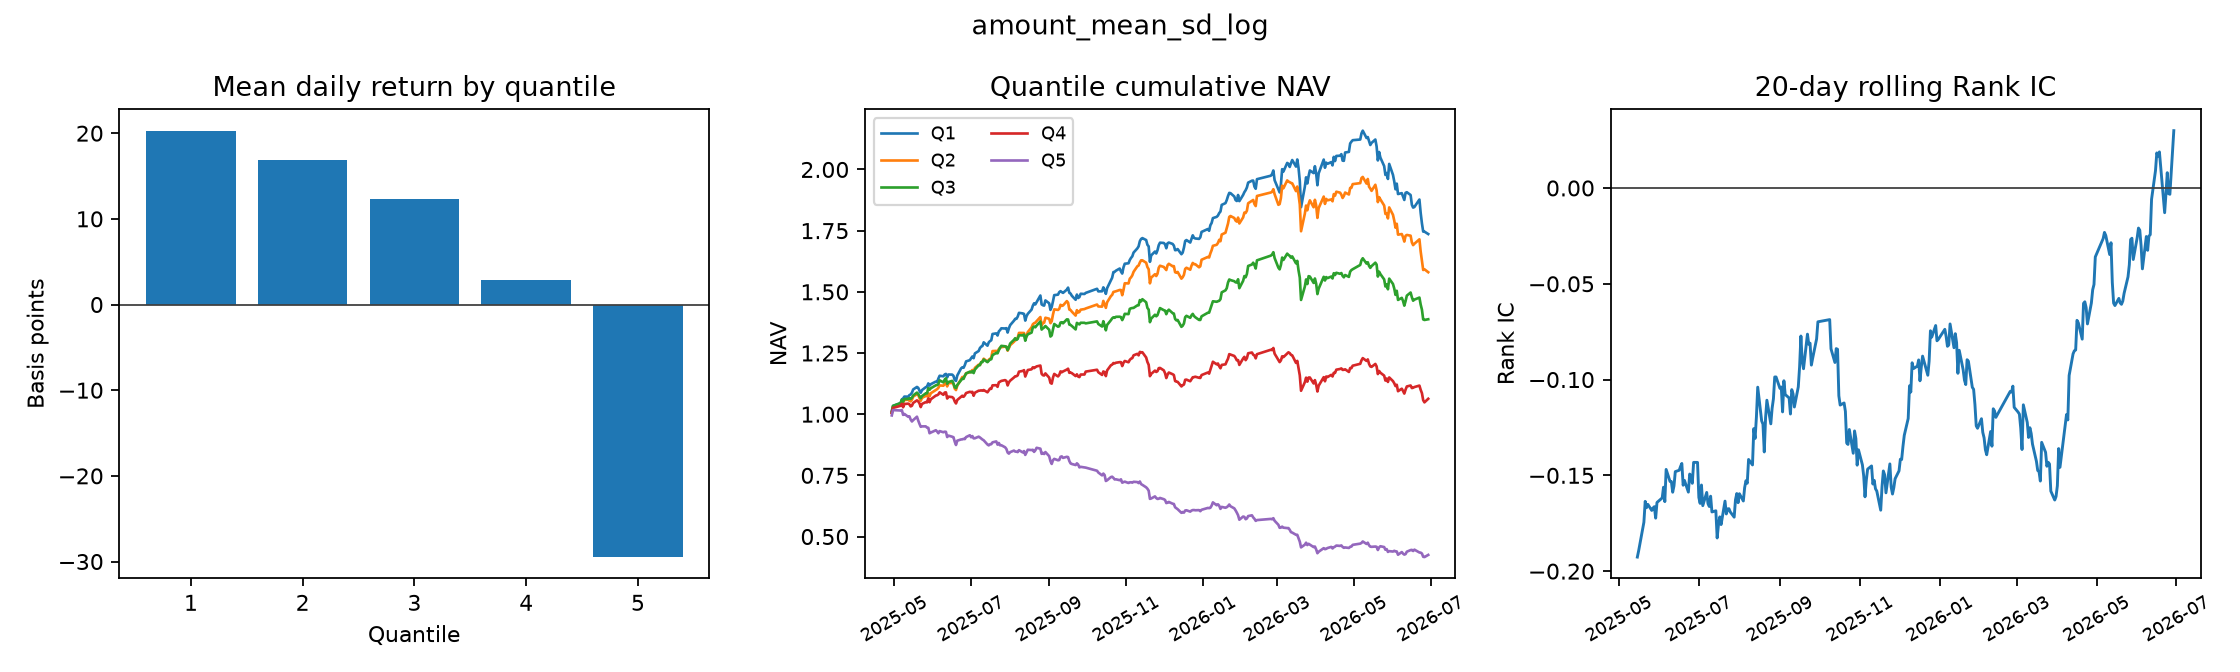
\includegraphics[width=0.96\textwidth]{qr_factor_amount.png}
\caption{Diagnostics for the multi-window dispersion of average turnover. The negative Rank IC and declining portfolio returns indicate that this factor should be used with its sign reversed.}
\end{figure}

\begin{figure}[H]\centering
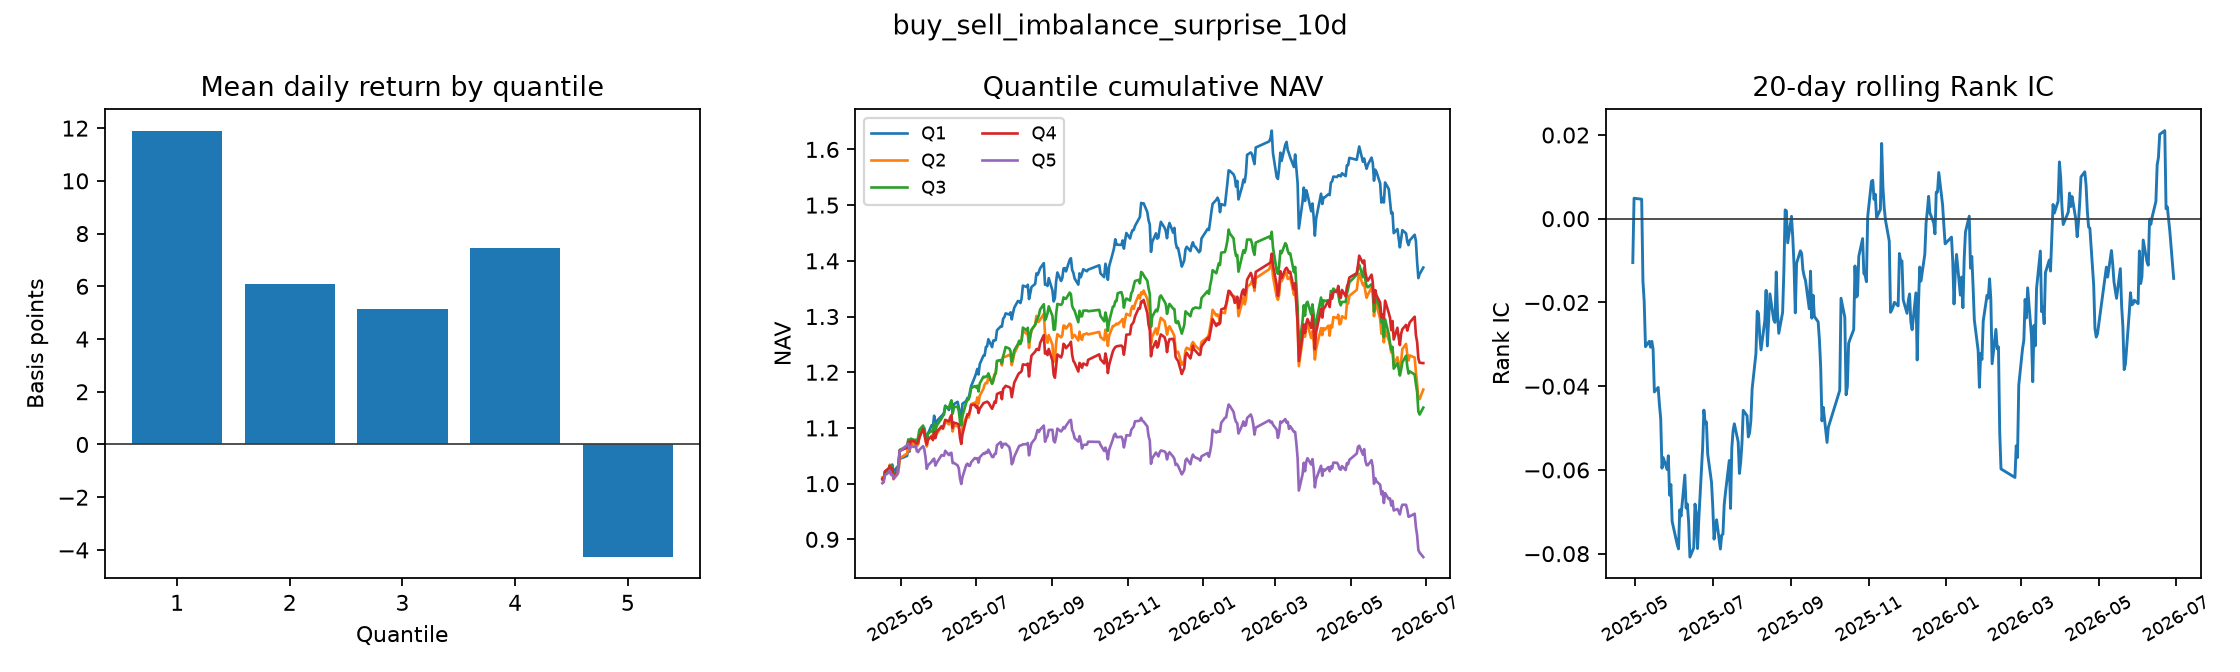
\includegraphics[width=0.96\textwidth]{qr_factor_imbalance.png}
\caption{Diagnostics for aggressive buy--sell imbalance. Its Rank IC is close to zero and its standalone predictive power is weak, so it should not determine the portfolio direction by itself.}
\end{figure}

\begin{figure}[H]\centering
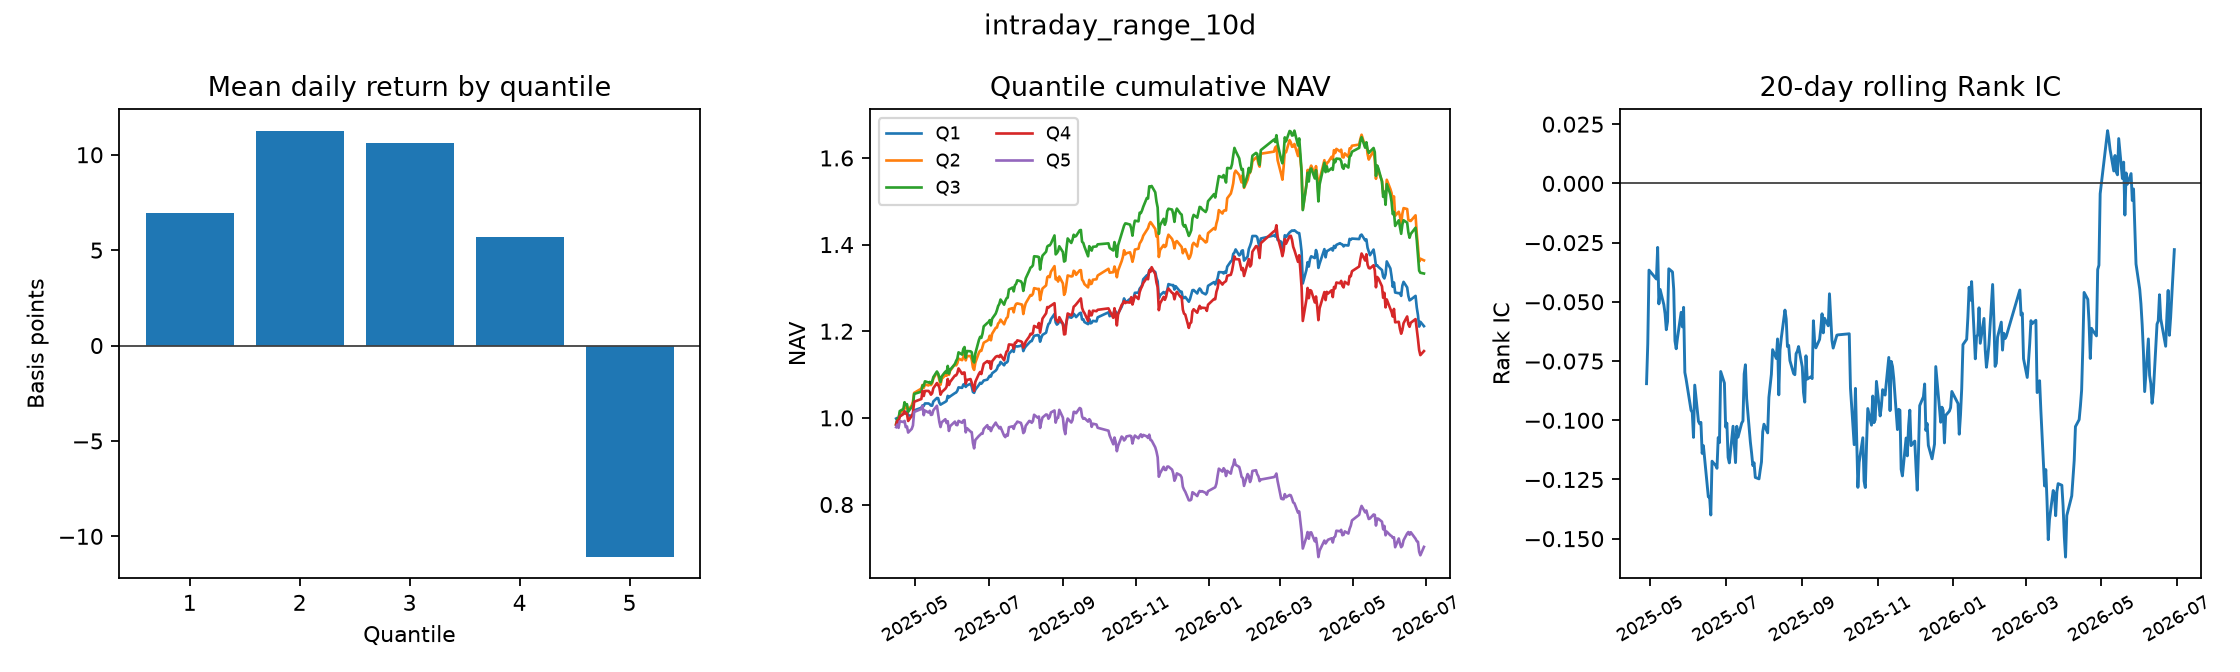
\includegraphics[width=0.96\textwidth]{qr_factor_range.png}
\caption{Diagnostics for the 10-day intraday range. High-range groups have weaker subsequent returns, making this a stable negative factor.}
\end{figure}

\begin{figure}[H]\centering
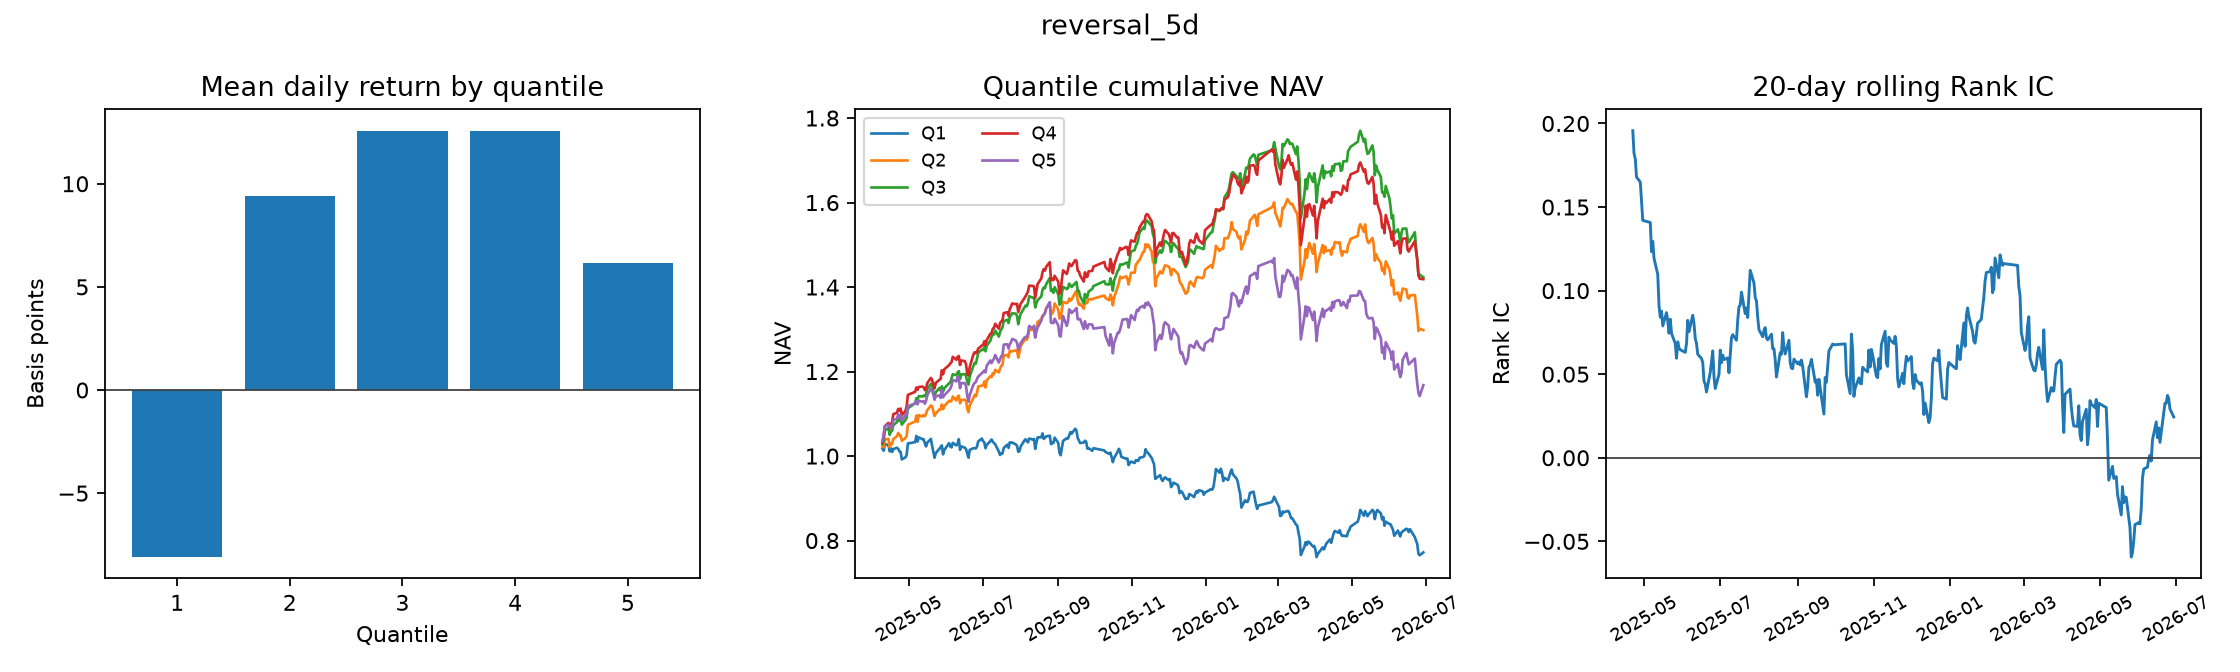
\includegraphics[width=0.96\textwidth]{qr_factor_reversal.png}
\caption{Diagnostics for the 5-day reversal factor. Positive Rank IC and positive long--short returns indicate that recently weak stocks experience some subsequent rebound.}
\end{figure}

\begin{figure}[H]\centering
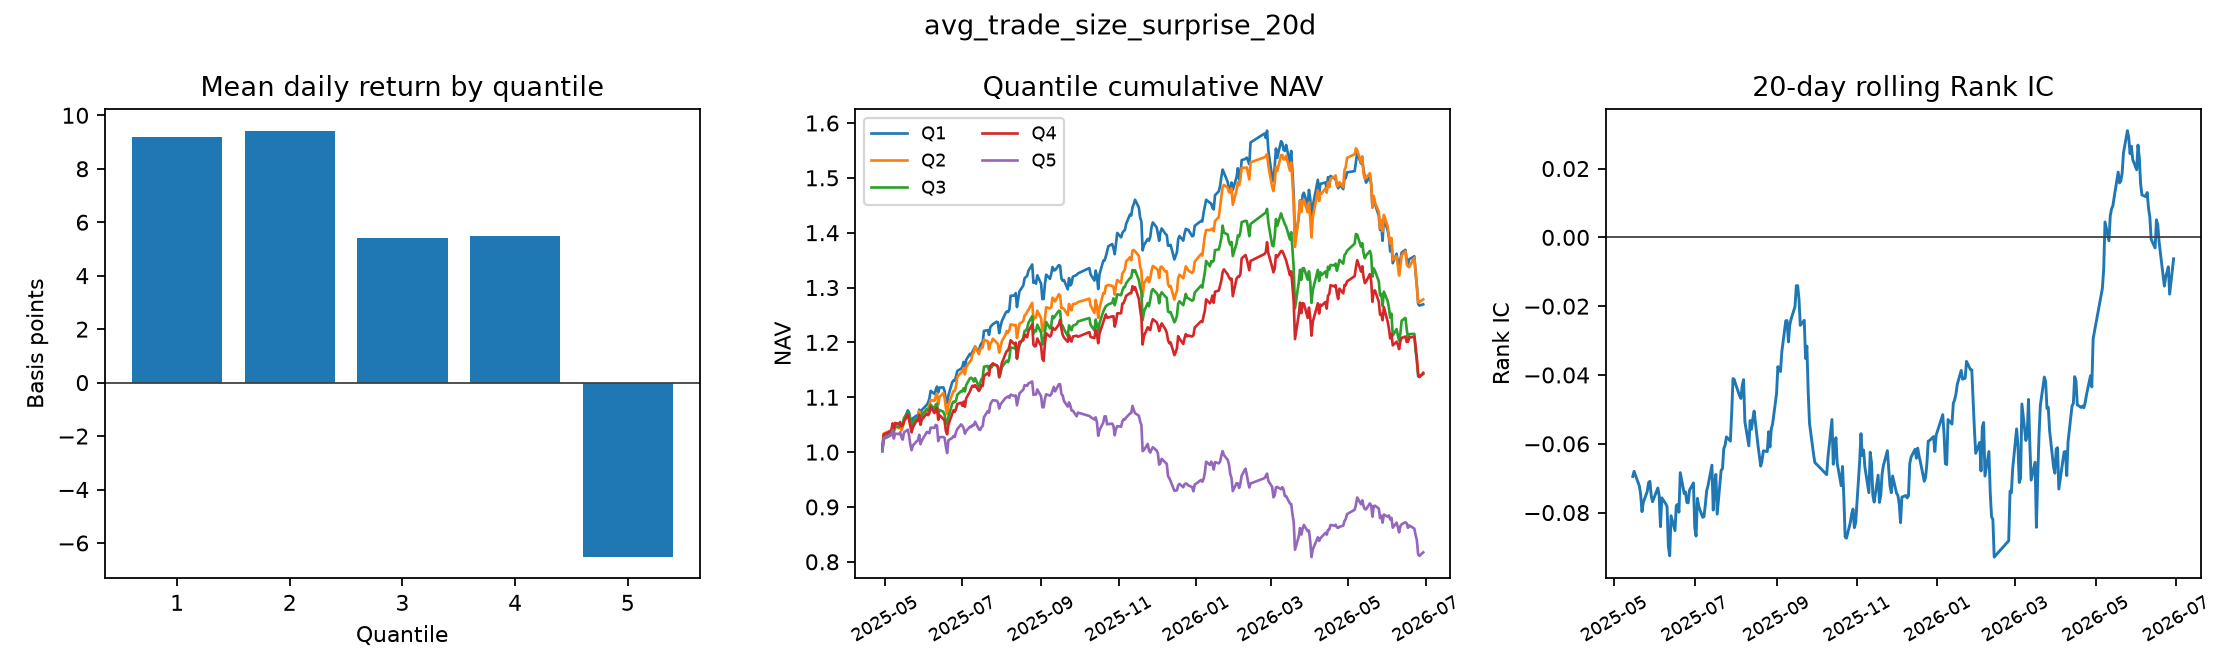
\includegraphics[width=0.96\textwidth]{qr_factor_trade_size.png}
\caption{Diagnostics for the 20-day abnormal average trade-size factor. Unusually large average trade size is negatively correlated with next-day returns.}
\end{figure}

\begin{figure}[H]\centering
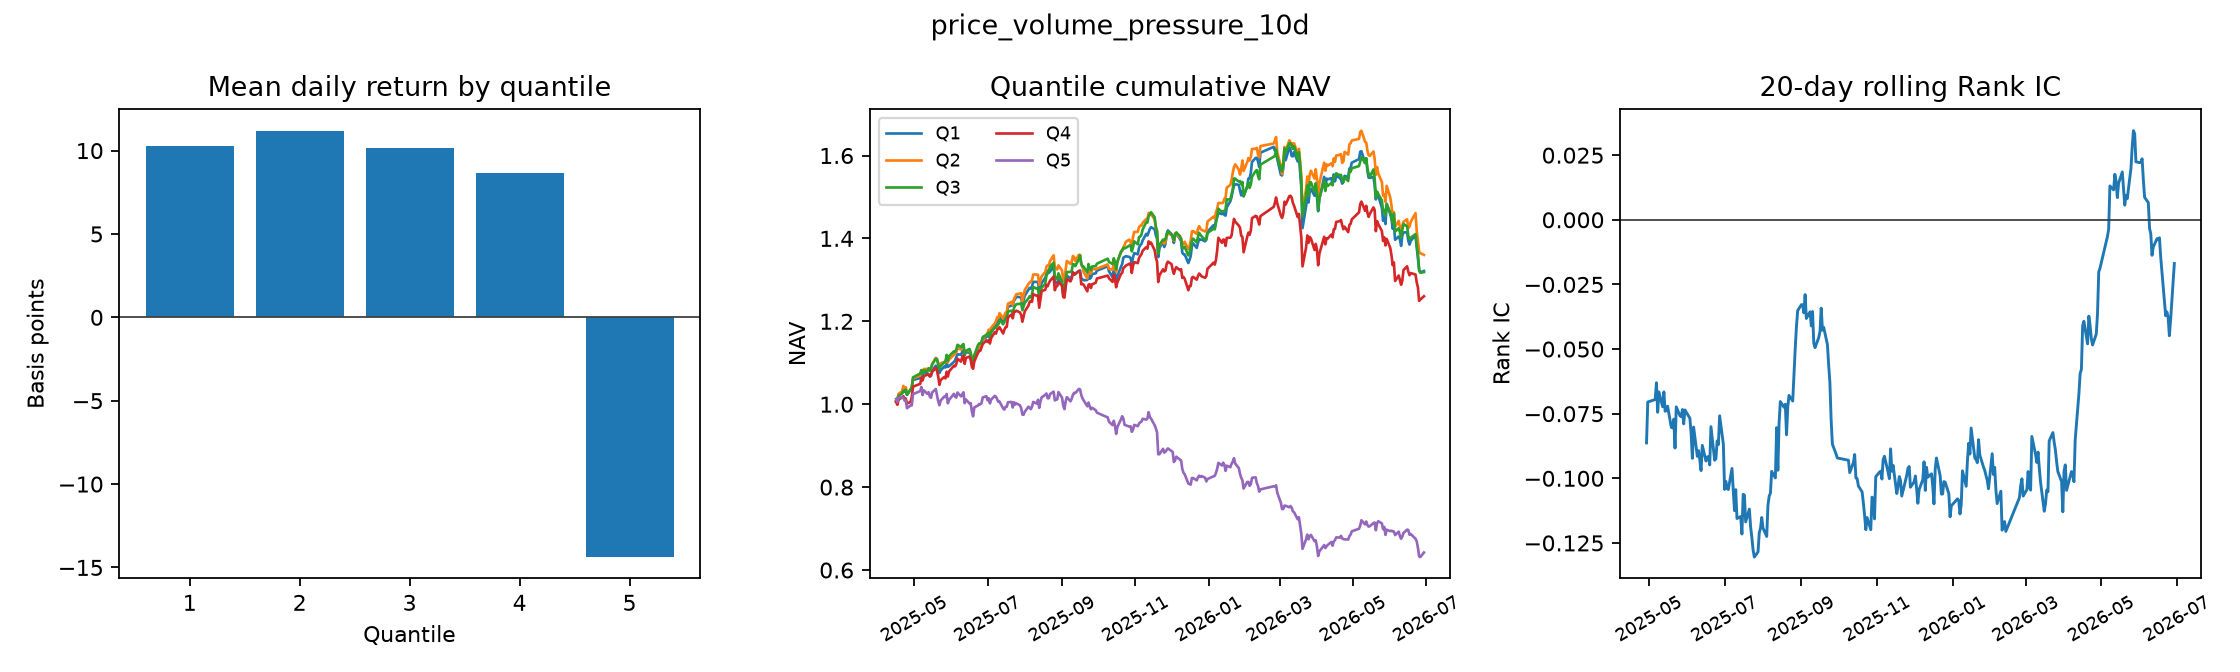
\includegraphics[width=0.96\textwidth]{qr_factor_price_volume.png}
\caption{Diagnostics for the 10-day price--volume pressure factor. Its predictive direction is negative, suggesting that recent same-direction price and volume pressure may be followed by a correction.}
\end{figure}

\begin{figure}[H]\centering
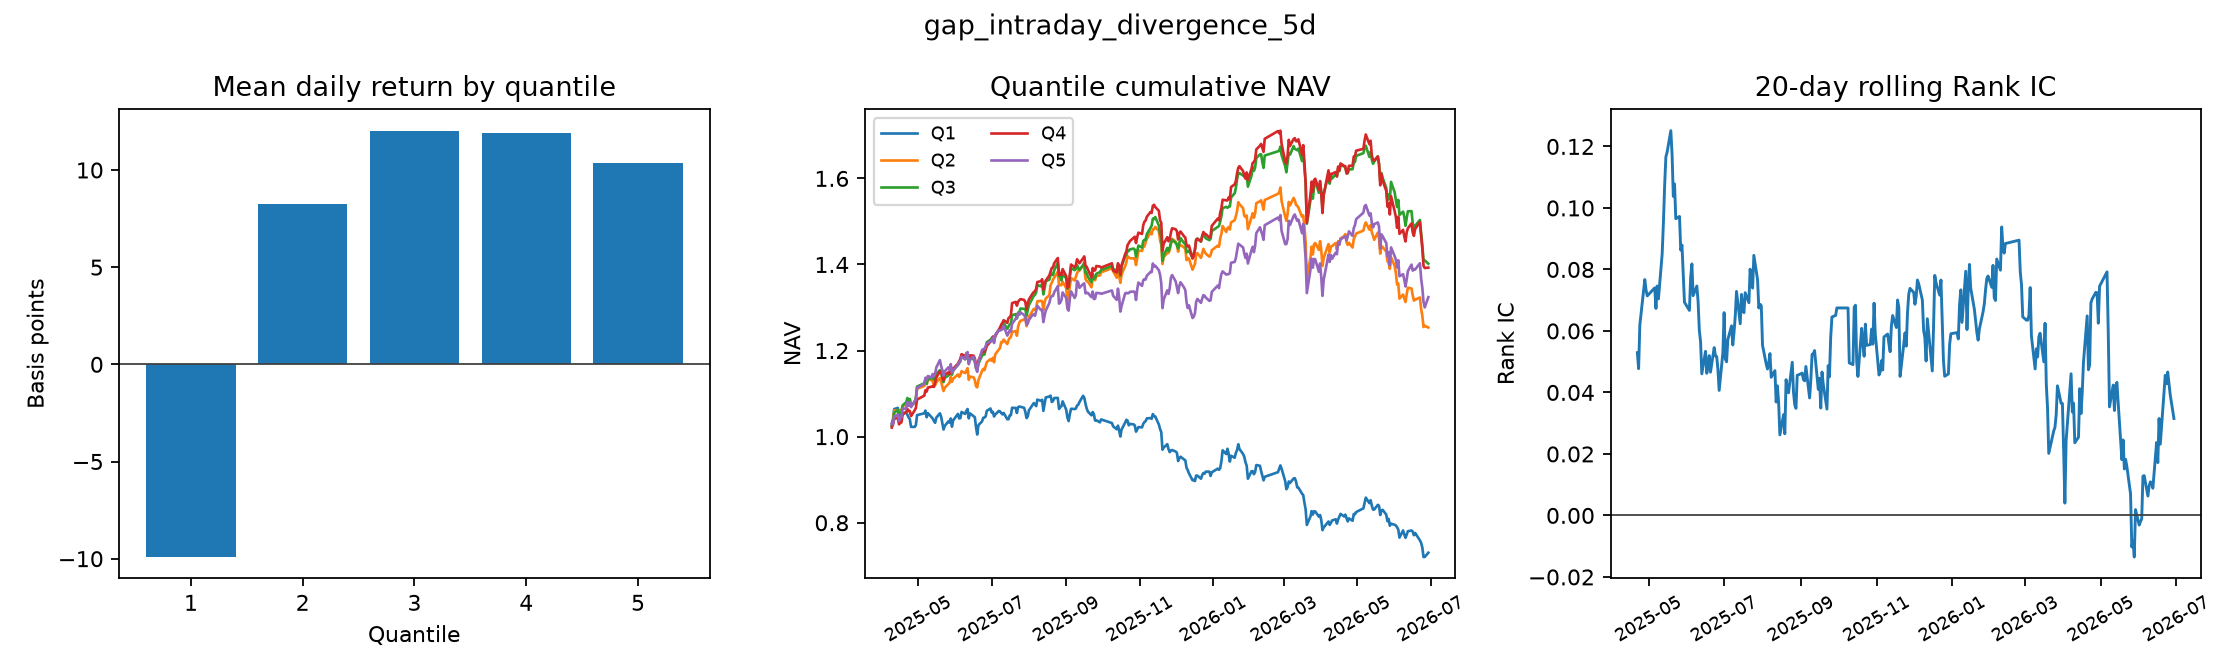
\includegraphics[width=0.96\textwidth]{qr_factor_gap_intraday.png}
\caption{Diagnostics for the 5-day overnight--intraday return-divergence factor. Its Q5--Q1 cumulative return is 80.41\%, the strongest among the newly added factors.}
\end{figure}

\section{Correlation and Long--Short Net Value}

Factor correlations are used to identify duplicated information. Among the 18 factors, idiosyncratic volatility and ordinary realized volatility have a correlation of approximately -0.959, showing substantial overlap in their risk information. The new risk factors therefore cannot be added mechanically to the formal signal on the basis of standalone IC. Because the full risk-factor combination worsens drawdown in the holdout period, the final specification retains the original 15-factor ranking and uses only a separate portfolio-volatility target.

\begin{figure}[H]\centering
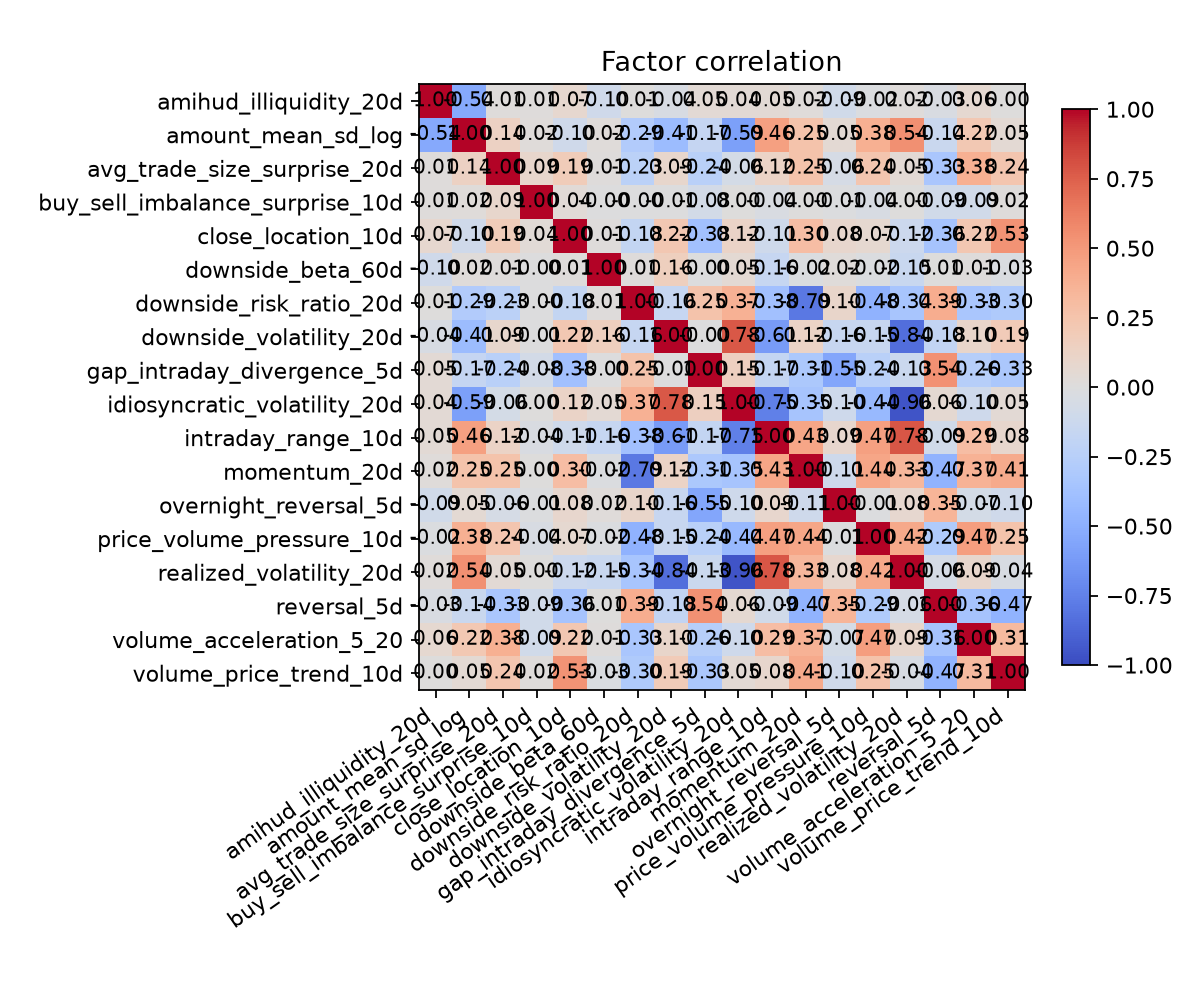
\includegraphics[width=0.86\textwidth]{qr_factor_corr.png}
\caption{Heatmap of cross-sectional correlations among the 18 factors. The new risk factors overlap visibly with conventional volatility measures.}
\end{figure}

\begin{figure}[H]\centering
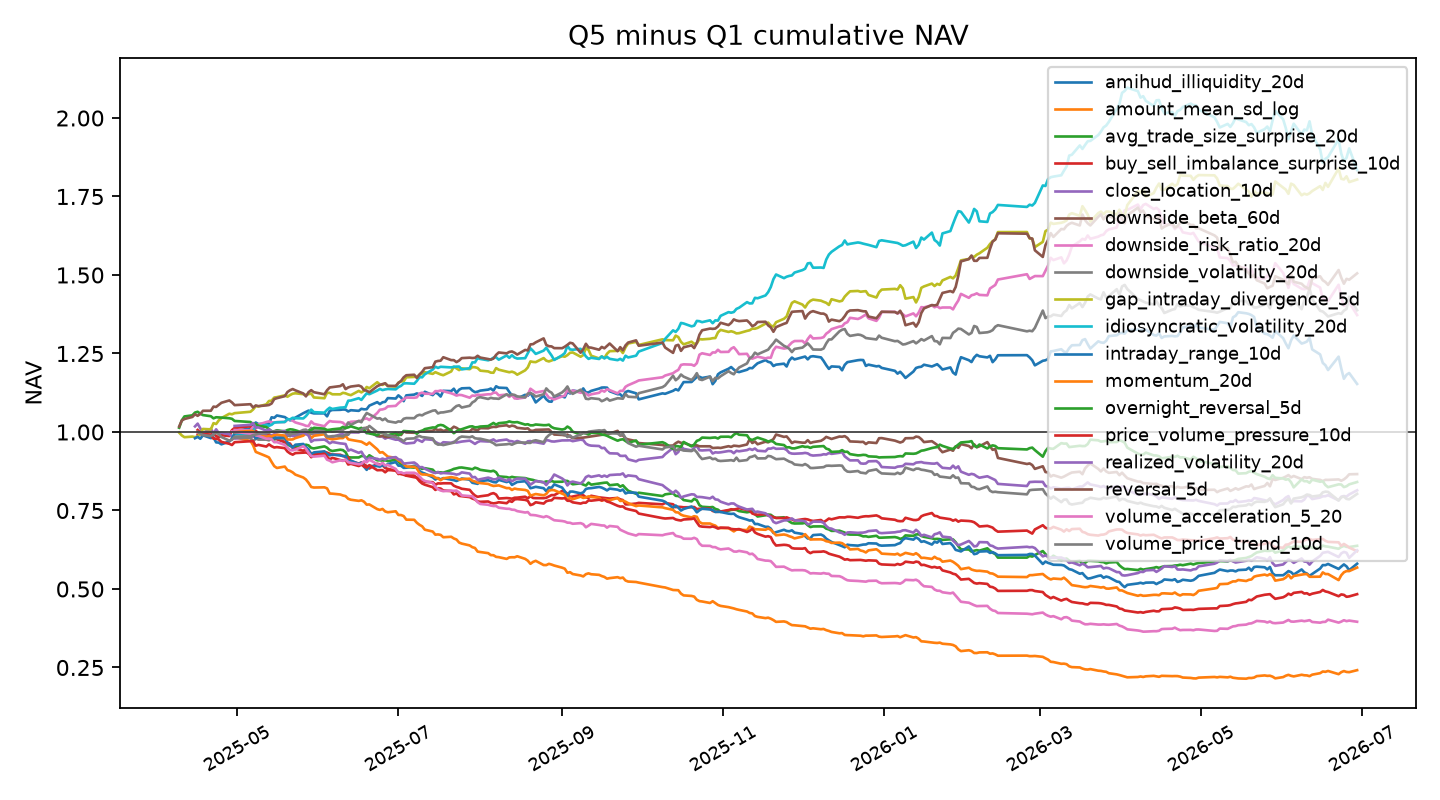
\includegraphics[width=0.94\textwidth]{qr_factor_ls_nav.png}
\caption{Cumulative net values of the 18 factor Q5--Q1 long--short portfolios. Factors with different predictive signs are reoriented according to historical IC before combination.}
\end{figure}

\chapter[Portfolio Construction and Look-Ahead-Free Backtesting]{Portfolio Construction and\\Look-Ahead-Free Backtesting}

\section{Composite Signal Based on Historical-IC Weights}

For factor $k$, the direction and weight on trading day $t$ use only the 20-day historical IC available through $t-1$:
\begin{equation}
\bar{IC}_{k,t}=\frac{1}{20}\sum_{s=t-20}^{t-1}IC_{k,s},\qquad
w_{k,t}=\frac{\bar{IC}_{k,t}}{\sum_j |\bar{IC}_{j,t}|}.
\end{equation}
The composite score is
\begin{equation}
Score_{i,t}=\sum_k w_{k,t}z_{i,k,t}.
\end{equation}
The quantity $IC_{k,t}=\mathrm{corr}(F_{k,t},R_{t+1})$ cannot be used directly to determine trades on day $t$, because $R_{t+1}$ has not yet occurred when orders are submitted.

\section{Candidate Risk Weights and the Adopted Rule}

To reduce risk, the research additionally tests 60-day exponentially weighted ICIR weights. Using only the IC history available through $t-1$,
\begin{equation}
q_{k,t}=\frac{\mathrm{EWMA}_{60}(IC_{k,s},\,s\le t-1)}{\mathrm{EWSD}_{60}(IC_{k,s},\,s\le t-1)},\qquad
\tilde q_{k,t}=\mathrm{clip}(q_{k,t},-0.25,0.25).
\end{equation}
Positive factor scores are divided by each stock's prior 20-day volatility, and individual target weights are capped at 4\%. Execution constraints remain unchanged: positions that cannot be sold remain frozen rather than being forcibly normalized away.

The complete replacement of factors and IC weights lowers volatility but materially worsens holdout drawdown. The adopted specification therefore preserves the original 15-factor signal and adds only a dynamic volatility target. Let $r^{gross}_{p,s}$ be realized gross portfolio returns available before day $t$:
\begin{equation}
\widehat\sigma_{p,t}=\mathrm{SD}(r^{gross}_{p,t-20},\ldots,r^{gross}_{p,t-1})\sqrt{252},\qquad
L_t=\mathrm{clip}\left(\frac{15\%}{\widehat\sigma_{p,t}},0.5,1.0\right).
\end{equation}
If the 20-day history is unavailable, $L_t=1$. This overlay uses only realized past returns and therefore introduces no same-day or future information.

\section{Turnover Control and Holding Rules}

The portfolio holds 30 stocks and rebalances every five trading days. A current holding is retained as long as it remains in the top 60 of the composite ranking; the portfolio is then replenished to 30 stocks from the latest ranking. This buffer prevents small changes between ranks 30 and 31 from automatically triggering trades.

\begin{figure}[H]\centering
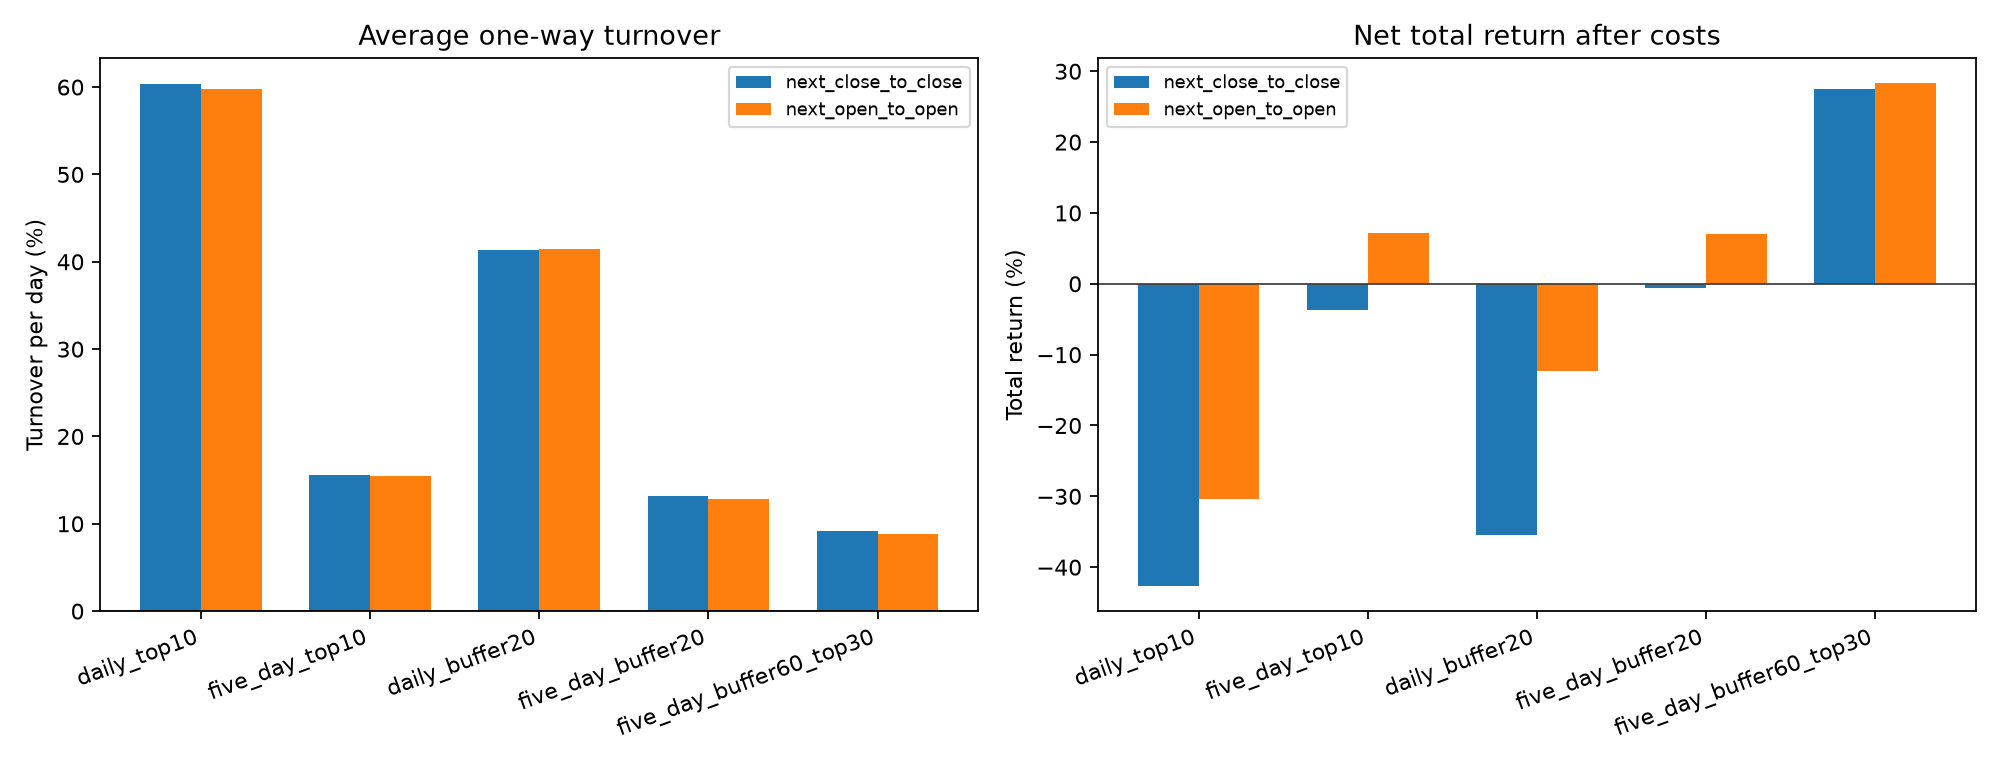
\includegraphics[width=0.96\textwidth]{qr_turnover_comparison.png}
\caption{Comparison of turnover-control policies. Under next-day-open execution, average daily one-way turnover is 8.81\%.}
\end{figure}

\section{Execution Timing, Constraints, and Transaction Costs}

A signal is formed on day $t$ and can only be executed at the open or close of day $t+1$, after which the position is held until the next corresponding price point. Zero volume or turnover indicates a suspension. A stock at a one-price upper limit cannot be purchased, while a stock at a one-price lower limit cannot be sold. Positions that cannot be sold remain in the portfolio.

\noindent Transaction costs have three components: a five-basis-point commission on sell value; five basis points of baseline slippage on both buys and sells; and square-root market impact driven by the order value as a fraction of daily turnover:
\begin{equation}
c^{impact}_{i,t}=\min\left(c_{max},\eta\sqrt{\frac{Q_{i,t}}{ADV_{i,t}}}\right).
\end{equation}
Here, $Q$ is order value, $ADV$ is daily turnover, and $\eta$ is the impact coefficient. This design assigns higher costs to less liquid stocks and larger orders.

\chapter{Risk--Return Results and Robustness Tests}

\section{Definitions of Performance Metrics}

Cumulative return is $\prod_t(1+r_t)-1$; annualized return is $(1+R)^{252/T}-1$; annualized volatility is $\sigma(r)\sqrt{252}$; maximum drawdown is the largest decline in net value relative to its historical peak; the Sharpe ratio is the annualized average return in excess of the risk-free rate divided by annualized volatility; and the information ratio is the annualized mean active return divided by tracking error. The equal-weight benchmark uses the same-day equal-weight return of stocks that can be purchased on the entry date.

\begin{table}[H]
\centering
\caption{Full-sample risk--return results of the final strategy}
\begin{tabular}{lrr}
\toprule
Metric & Next-day close & Next-day open \\
\midrule
Cumulative return before costs & 37.97\% & 38.33\% \\
Cumulative return after costs & 27.52\% & 28.30\% \\
Annualized return & 24.96\% & 25.66\% \\
Annualized excess return & 20.65\% & 23.02\% \\
Annualized volatility & 18.84\% & 18.50\% \\
Maximum drawdown & -11.93\% & -10.90\% \\
Sharpe ratio & 1.277 & 1.327 \\
Information ratio & 1.880 & 1.838 \\
Average daily one-way turnover & 9.22\% & 8.81\% \\
Total transaction costs & 951,129 & 911,060 \\
\bottomrule
\end{tabular}
\end{table}

\begin{figure}[H]\centering
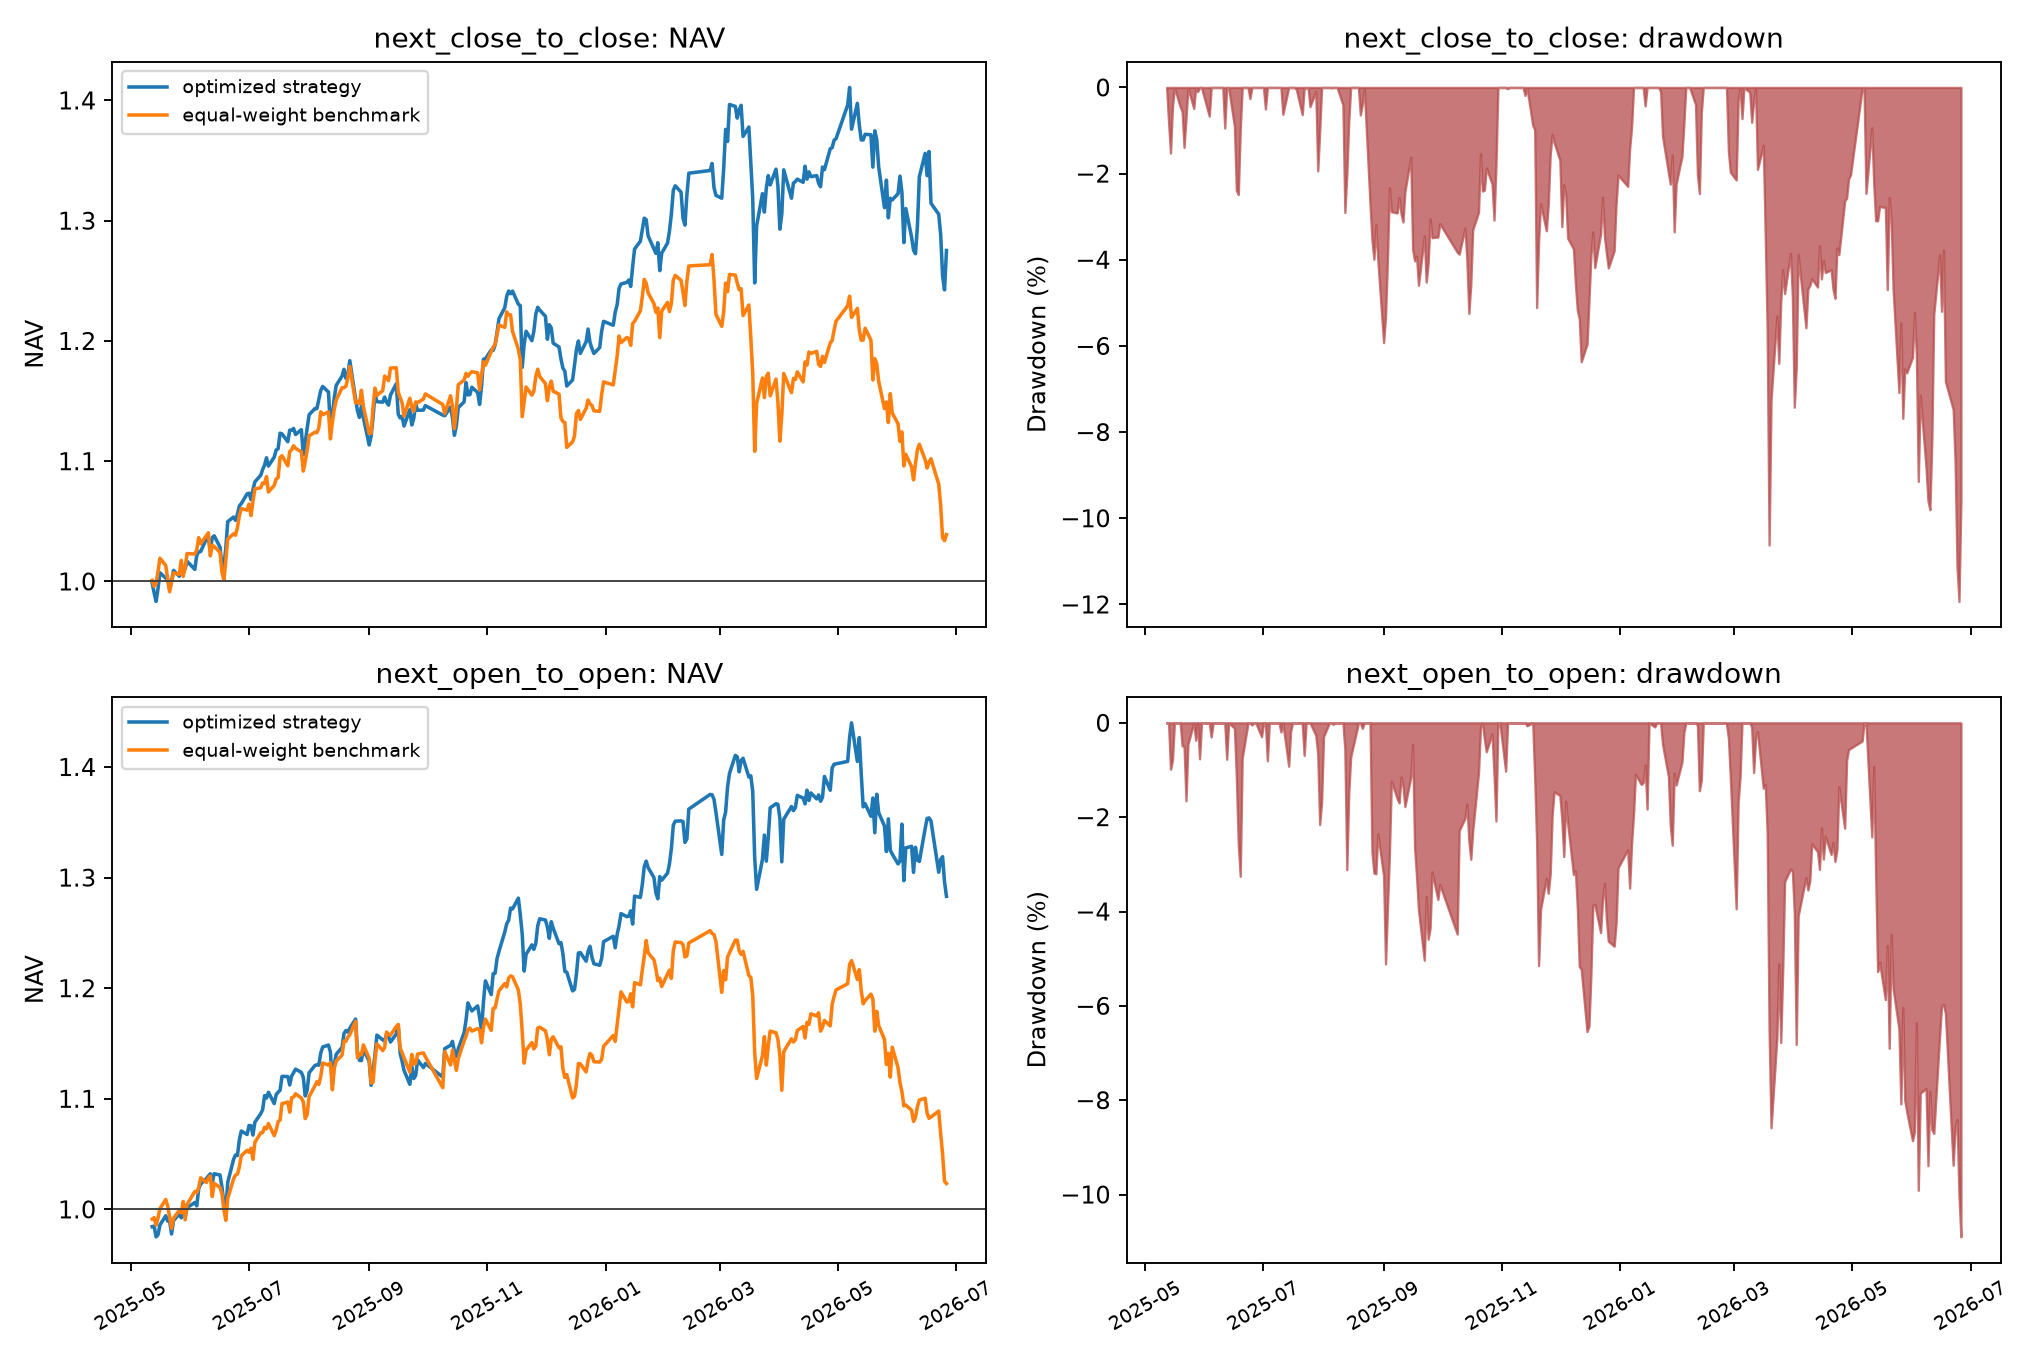
\includegraphics[width=0.98\textwidth]{qr_nav_drawdown.png}
\caption{Net value of the formal factor strategy, equal-weight benchmark, and drawdown. Next-day-open execution outperforms next-day-close execution in both return and drawdown.}
\end{figure}

\begin{figure}[H]\centering
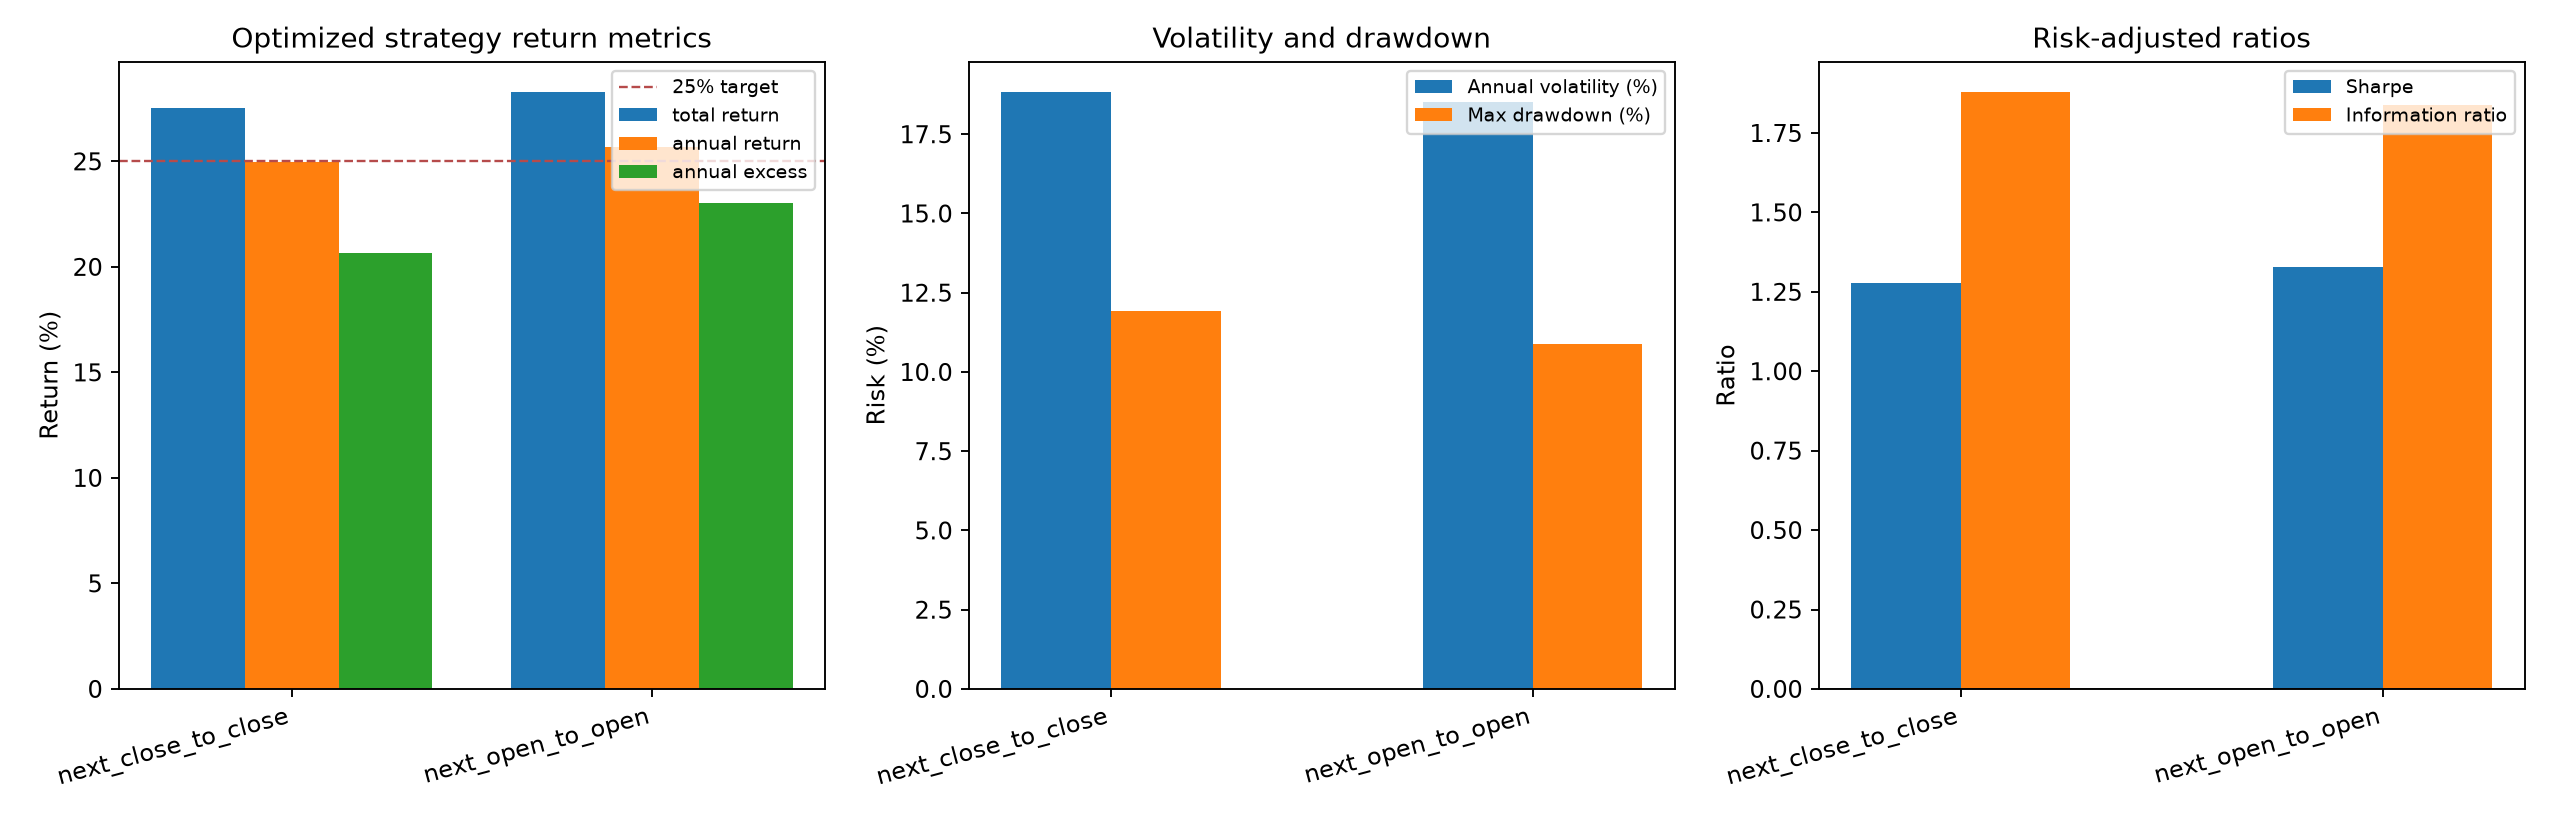
\includegraphics[width=0.96\textwidth]{qr_risk_metrics.png}
\caption{Side-by-side comparison of return, volatility, drawdown, Sharpe ratio, information ratio, and turnover.}
\end{figure}

\section{15\% Volatility Target and Risk Decomposition}

The table directly compares the original 15-factor signal at unit exposure, a fixed 1.24-times exposure, and the adopted 15\% volatility target. In the full sample, the dynamic target gives up about 0.71 percentage points of annualized return relative to the unit-exposure baseline while reducing annualized volatility from 18.50\% to 16.33\% and improving maximum drawdown from -10.90\% to -9.58\%. Its risk improvement is even clearer relative to the fixed 1.24-times exposure.

\begin{table}[H]
\centering
\small
\caption{Next-day-open risk-budget comparison}
\resizebox{\textwidth}{!}{%
\begin{tabular}{llrrrr}
\toprule
Sample & Version & Cumulative Return & Annualized Return & Annualized Volatility & Maximum Drawdown \\
\midrule
Full sample & Original signal, 1.00x & 28.30\% & 25.66\% & 18.50\% & -10.90\% \\
Full sample & Fixed 1.24x exposure & 33.30\% & 30.13\% & 22.94\% & -13.60\% \\
Full sample & 15\% volatility target & 27.52\% & 24.95\% & 16.33\% & -9.58\% \\
\midrule
Final 20\% holdout & Original signal, 1.00x & -5.16\% & -21.54\% & 23.06\% & -10.90\% \\
Final 20\% holdout & Fixed 1.24x exposure & -6.79\% & -27.54\% & 28.58\% & -13.60\% \\
Final 20\% holdout & 15\% volatility target & -4.10\% & -17.44\% & 18.35\% & -9.58\% \\
\bottomrule
\end{tabular}%
}
\end{table}

\begin{figure}[H]\centering
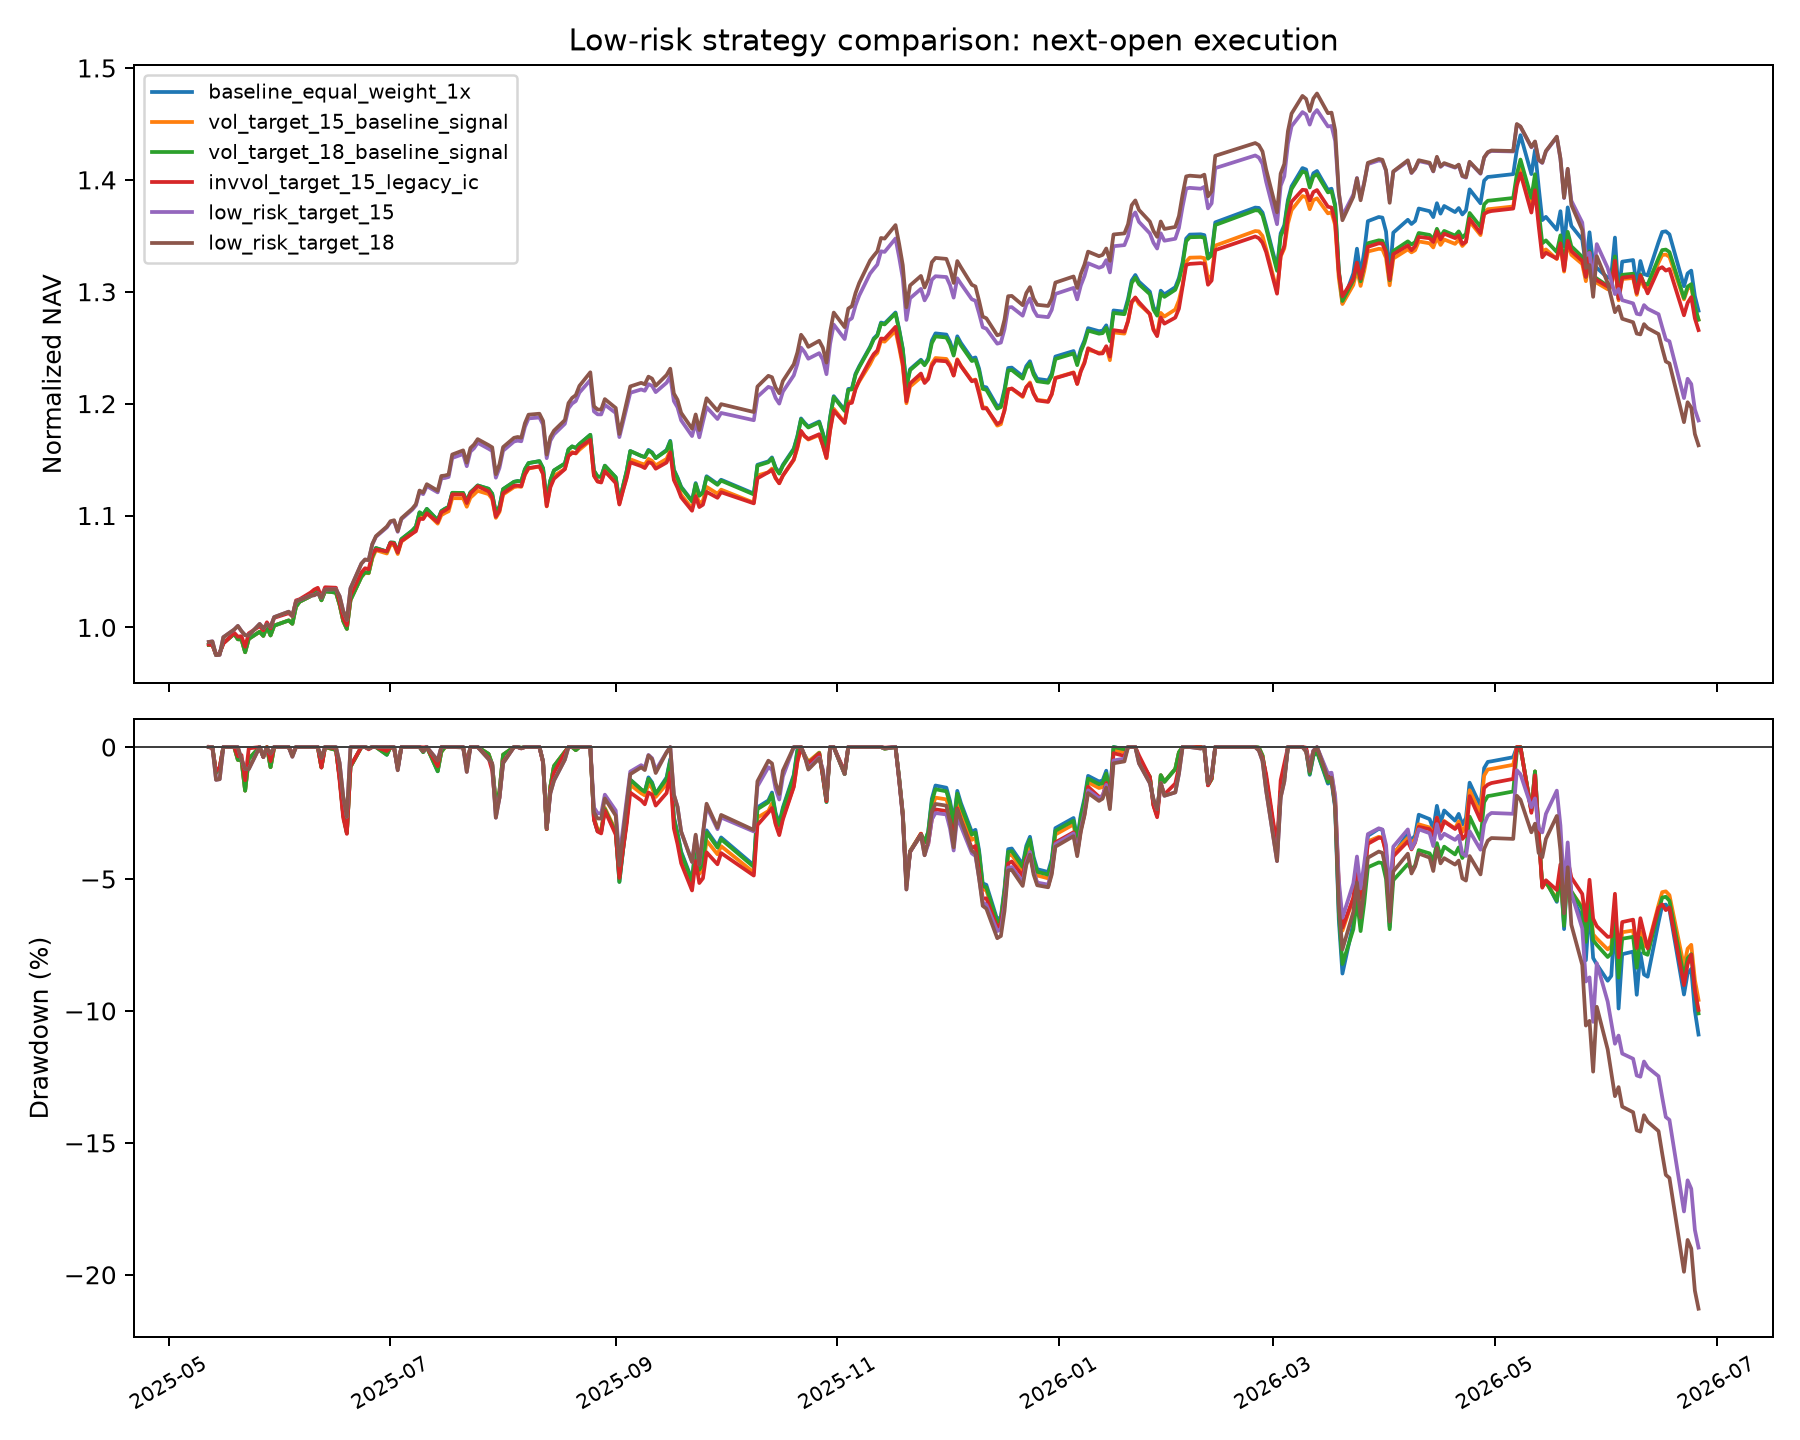
\includegraphics[width=0.98\textwidth]{qr_low_risk_nav_drawdown.png}
\caption{Net-value and drawdown decomposition across risk-control versions. Replacing the full factor and IC-weighting system lowers volatility but worsens holdout drawdown; the adopted version preserves the original signal and applies the 15\% volatility target.}
\end{figure}

\section{Research and Holdout Periods}

To distinguish research-selection effects from temporal generalization, the sample is split chronologically into the first 80\% as the research period and the final 20\% as the holdout period. The adopted 15\% volatility-target strategy returns 32.97\% in the research period and -4.10\% in the holdout period. The equal-weight benchmark returns -10.44\% over the holdout period, so cumulative active return is 7.08\%. This result indicates relative resilience in a declining market but does not demonstrate stable positive absolute returns.

\begin{figure}[H]\centering
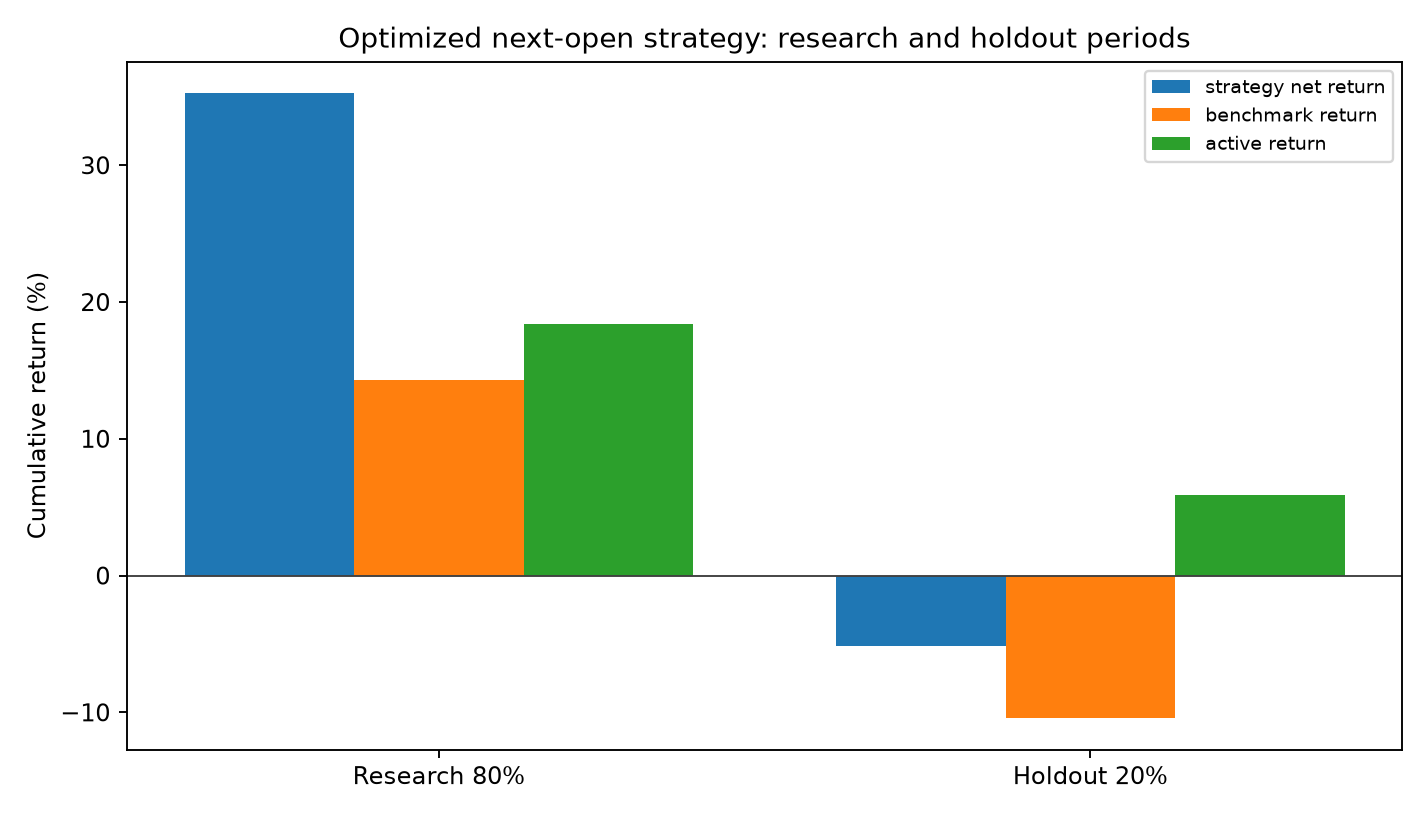
\includegraphics[width=0.96\textwidth]{qr_period_split.png}
\caption{Comparison of the full sample, the first 80\% research period, and the final 20\% holdout period for the adopted 15\% volatility-target strategy. The full-sample return of 27.52\% is not a substitute for strict out-of-sample validation.}
\end{figure}

\clearpage
\subsubsection{Sample-Period Partition and Definitions}

The complete dataset is split chronologically into a research period and a final holdout period. The research period is used for factor exploration, model fitting, parameter selection, and validation; the validation period is therefore part of the research period. Because the final 20\% holdout was used to compare risk-control versions in this study, it is quasi-out-of-sample rather than a strictly independent OOS test. ``Out-of-sample'' describes an evaluation method: the relevant predictions or returns come from data not used to fit the current model or select its parameters. It is not a fixed partition alongside the full sample, research period, validation period, and holdout period. Full-sample results contain both the research and holdout periods and are presented only as an overall backtest, not as independent out-of-sample evidence.

\begin{table}[H]
\centering
\caption{Unified definitions of sample periods}
\small
\begin{tabularx}{\textwidth}{
    >{\raggedright\arraybackslash}p{3.2cm}
    >{\raggedright\arraybackslash}X
    >{\raggedright\arraybackslash}X
}
\toprule
Term & Definition & Purpose \\
\midrule
Full Sample
& All dates covered by the report, including the research period and the final holdout period
& Present overall net value, returns, drawdown, and transaction costs \\

Research Period
& Interval used for factor exploration, strategy design, model fitting, and parameter selection
& Determine factors, number of holdings, rebalance frequency, buffer, and cost parameters \\

Validation Period
& Interval within the research period used for model selection, hyperparameter selection, threshold selection, and early stopping
& Compare candidate approaches and determine the final configuration \\

Holdout Period
& Final chronological 20\% interval; used here to compare risk-control versions
& Provide a quasi-out-of-sample robustness check \\

Out-of-Sample
& A prediction or backtest uses data that were not involved in fitting the current model or selecting its parameters
& Describe walk-forward test windows or truly untouched future-period results \\
\bottomrule
\end{tabularx}
\end{table}

\subsubsection{Backtest Results by Period}

To distinguish research-selection effects from temporal generalization, the backtest results are reported separately for the research period, the final holdout period, and the full sample.

\begin{table}[H]
\centering
\small
\begin{threeparttable}
\caption{Backtest results by period}
\label{tab:period_backtest}
\renewcommand{\arraystretch}{1.5}
\begin{tabularx}{\textwidth}{
    >{\raggedright\arraybackslash}p{2.7cm}
    >{\raggedright\arraybackslash}X
    >{\centering\arraybackslash}p{2.0cm}
    >{\centering\arraybackslash}p{2.2cm}
    >{\centering\arraybackslash}p{2.0cm}
    >{\raggedright\arraybackslash}p{2.3cm}
}
\toprule
\textbf{Period}
& \textbf{Use of Data}
& \textbf{Strategy Cumulative Return}
& \textbf{Equal-Weight Benchmark Cumulative Return}
& \textbf{Cumulative Active Return}
& \textbf{Nature of Result} \\
\midrule

Research Period (First 80\%)
& Factor research, parameter selection, and strategy development
& 32.97\%
& 14.27\%
& 16.36\%
& Research-period result \\
\midrule

Holdout Period (Final 20\%)
& Risk-control version comparison
& -4.10\%
& -10.44\%
& 7.08\%
& Quasi-out-of-sample result\tnote{*} \\
\midrule

Full Sample
& Overall net-value and risk presentation
& 27.52\%
& 2.34\%
& 24.60\%
& Full-sample backtest result \\
\bottomrule
\end{tabularx}

\begin{tablenotes}[flushleft]
\footnotesize
\item[*]
Because the final 20\% holdout period was used to compare risk-control versions, this report labels it quasi-out-of-sample rather than strictly independent OOS. Active return is calculated from the strategy net value relative to the benchmark net value; it is not obtained by directly subtracting the two cumulative return percentages.
\end{tablenotes}
\end{threeparttable}
\end{table}

\noindent The adopted 15\% volatility-target strategy produces a cumulative return of 32.97\% in the research period and an absolute return of -4.10\% in the holdout period. The equal-weight benchmark returns -10.44\% over the same holdout period. The strategy therefore shows relative resilience in a declining market, but it has not yet demonstrated stable positive absolute returns.

\chapter{Multi-Stock Walk-Forward LSTM}

\section{Sample and Features}

The minute-level model uses six stocks and 140 trading days to predict whether the next minute's price will rise from the previous 20 minutes. Input features include log return, minute-level range, log volume, aggressive buy--sell imbalance, and intraday time position. The label is defined as
\begin{equation}
y_{t+1}=\mathbb{I}(C_{t+1}>C_t).
\end{equation}
Each sample contains only information available at or before the prediction time, preventing next-minute data from entering the input window.

\section{Expanding-Window Validation}

The model is a single-layer PyTorch LSTM with a hidden dimension of 16. Validation uses a three-fold expanding-window walk-forward scheme. Each fold contains at least 60 training days, 20 validation days, and 20 test days. Standardization parameters are estimated only from the training period, the validation period is used for model selection, and the three test windows do not overlap. The combined test windows contain 83,880 out-of-sample predictions, of which 31.09\% are positive-class observations.

\begin{table}[H]
\centering
\small
\caption{Out-of-sample classification results}
\begin{tabular}{lrrrrrrr}
\toprule
Model & Acc. & Bal. Acc. & Prec. & Recall & F1 & ROC AUC & PR AUC \\
\midrule
Majority class & 68.91\% & 50.00\% & 0.00\% & 0.00\% & 0.00\% & 0.5000 & 0.3109 \\
Logistic regression & 68.93\% & 51.23\% & 50.51\% & 4.40\% & 8.10\% & 0.6086 & 0.3993 \\
LSTM & 68.98\% & 52.28\% & 50.77\% & 8.10\% & 13.97\% & 0.6465 & 0.4276 \\
\bottomrule
\end{tabular}
\end{table}

\section{Accuracy and Interpretation}

Figure~\ref{fig:lstm-accuracy} presents combined out-of-sample accuracy and three-fold test accuracy in the same figure. The LSTM's overall accuracy is 68.98\%, but positive-class observations account for only 31.09\% of the sample. A majority-class model that always predicts a decline can therefore achieve 68.91\% accuracy. The LSTM improves on the majority-class baseline by only 0.07 percentage points, so 68.98\% cannot be interpreted directly as strong directional predictive power.

Balanced accuracy instead calculates recall separately for the positive and negative classes and then averages the two values. The LSTM's balanced accuracy is 52.28\%, higher than the majority-class baseline of 50.00\% and the logistic regression's 51.23\%. This indicates limited but positive incremental identification of minority-class upward observations. Test accuracies for the three folds are 69.22\%, 68.88\%, and 68.84\%, which are stable across time windows but remain very close to the majority-class baseline.

\begin{figure}[H]\centering
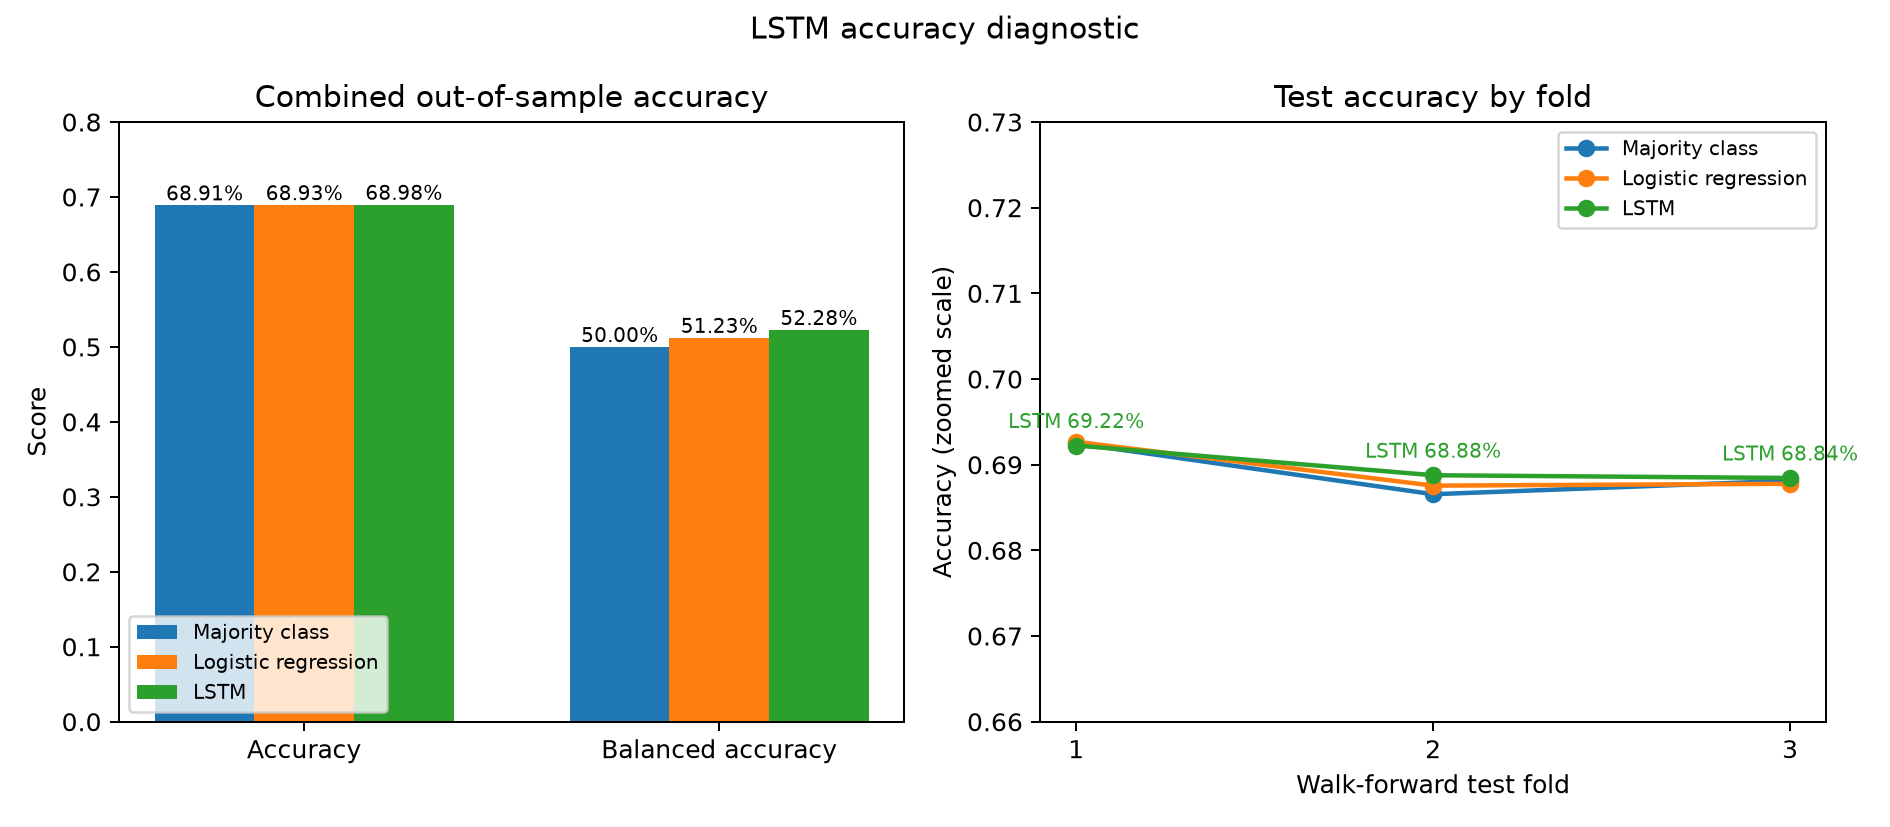
\includegraphics[width=0.98\textwidth]{qr_lstm_accuracy.png}
\caption{LSTM accuracy diagnostics. The left panel compares combined out-of-sample accuracy and balanced accuracy; the right panel compares test accuracy across the three folds. Because of class imbalance, overall accuracy must be interpreted together with the majority-class baseline, balanced accuracy, and ranking metrics.}
\label{fig:lstm-accuracy}
\end{figure}

Combining the positive-class recall of 8.10\%, ROC AUC of 0.6465, and PR AUC of 0.4276 yields a more complete conclusion: the LSTM ranks probabilities better than logistic regression, but at the 0.5 threshold it still misses many upward minutes. The model should currently be described as containing some out-of-sample ranking information, rather than as a high-accuracy or directly tradable minute-level strategy.

\begin{figure}[H]\centering
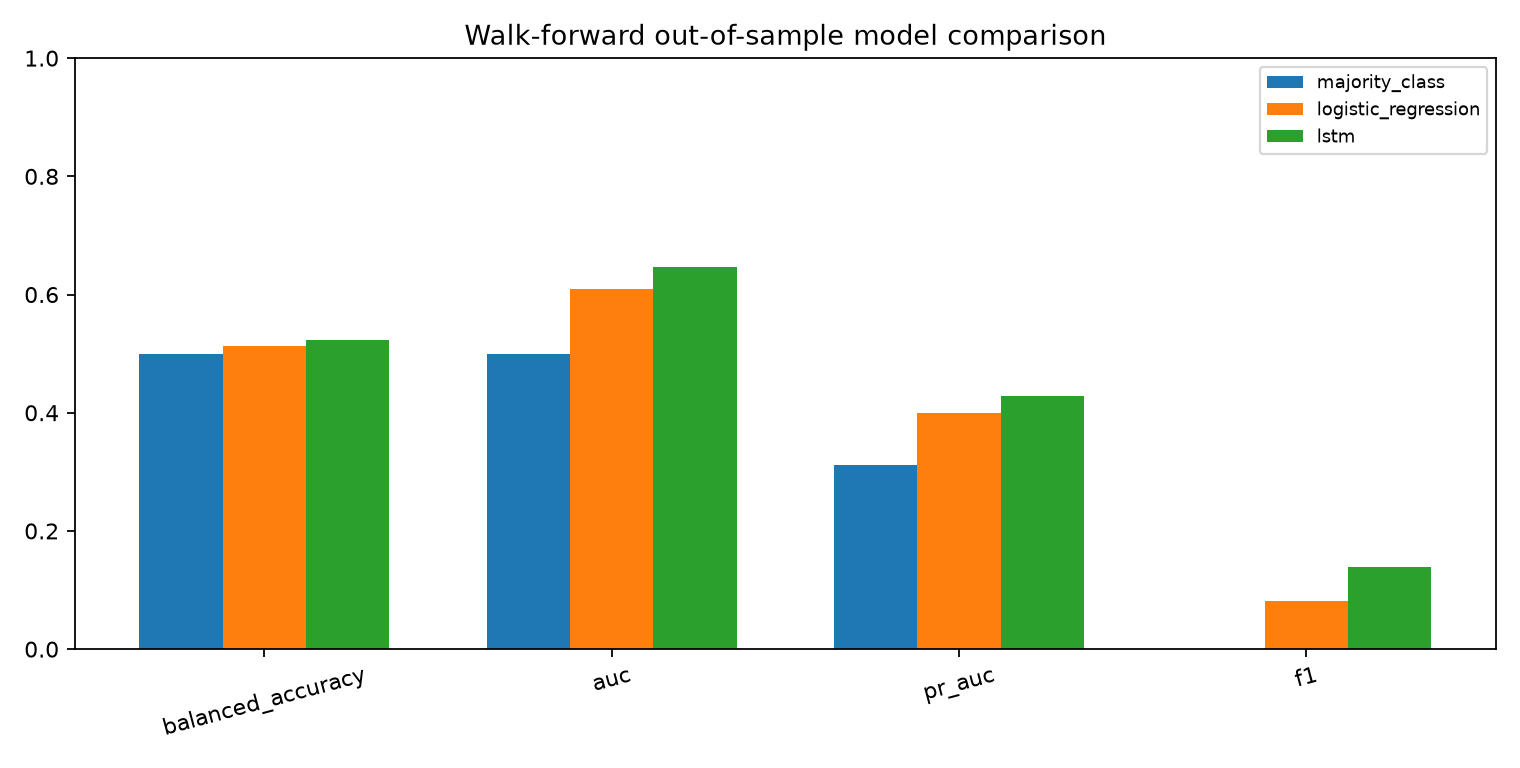
\includegraphics[width=0.88\textwidth]{qr_lstm_models.png}
\caption{Comparison of out-of-sample metrics for the majority-class model, logistic regression, and LSTM. The LSTM has stronger ranking metrics than logistic regression.}
\end{figure}

\begin{figure}[H]\centering
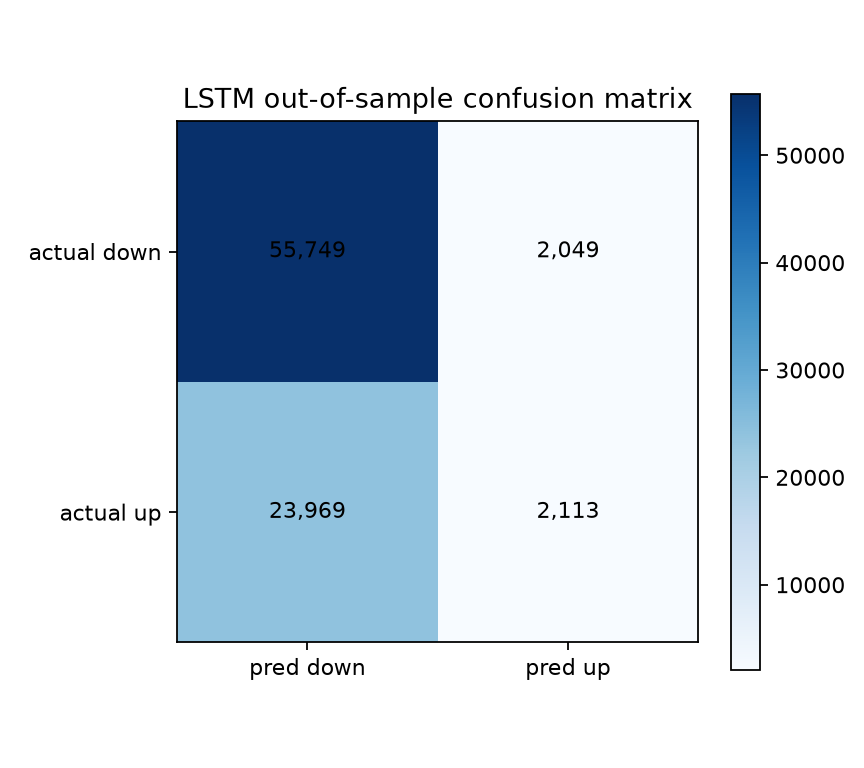
\includegraphics[width=0.72\textwidth]{qr_lstm_confusion.png}
\caption{Out-of-sample LSTM confusion matrix. There are 2,113 true positives and 23,969 false negatives, indicating low positive-class recall at the 0.5 threshold.}
\end{figure}

\begin{figure}[H]\centering
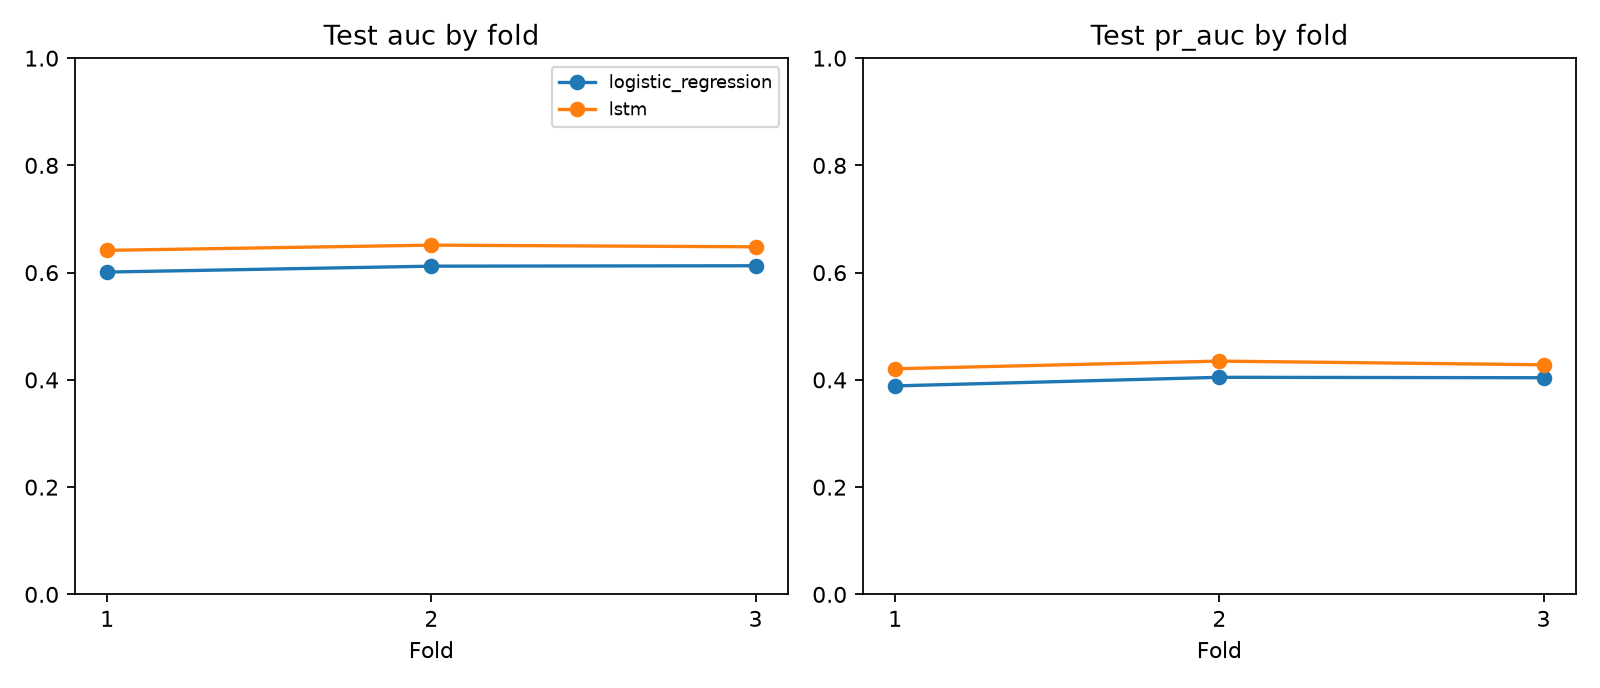
\includegraphics[width=0.92\textwidth]{qr_lstm_folds.png}
\caption{Per-fold metrics for the three-fold walk-forward evaluation. Fold-level results reveal whether performance is concentrated in a particular time window.}
\end{figure}

The LSTM's ROC AUC, PR AUC, and F1 score all exceed those of logistic regression, indicating that the sequence structure provides some additional ranking information. However, overall accuracy is almost identical to the majority-class baseline, and positive-class recall is only 8.10\%.

\chapter{Conclusion}

\begin{itemize}
  \item The project constructs 18 daily factors, including downside volatility, idiosyncratic volatility, and downside beta. Their standalone IC can be informative, but their high overlap with conventional volatility factors prevents mechanical inclusion in the formal signal.
  \item Historical-IC weighting prevents leakage from same-day future returns. The adopted rule preserves the original 15-factor ranking and applies a 15\% volatility target with exposure bounded between 0.5 and 1.0.
  \item Under next-day-open execution, the adopted strategy's full-sample cumulative return after costs is 27.52\%, annualized return is 24.95\%, annualized volatility is 16.33\%, maximum drawdown is -9.58\%, and Sharpe ratio is 1.446.
  \item The final 20\% holdout period returns -4.10\% versus -10.44\% for the equal-weight benchmark. Because this period was used to compare strategy versions, it is quasi-out-of-sample; strict OOS evidence requires a completely untouched future interval.
  \item The LSTM's out-of-sample ranking metrics exceed those of logistic regression, but its positive-class recall is low at the 0.5 threshold.
\end{itemize}

\end{document}
